\documentclass{article}

% if you need to pass options to natbib, use, e.g.:
%     \PassOptionsToPackage{numbers, compress}{natbib}
% before loading neurips_2026

% The authors should use one of these tracks.
% Before accepting by the NeurIPS conference, select one of the options below.
% 0. "default" for submission
%\usepackage{neurips_2026}
\usepackage[position]{neurips_2026}
% the "default" option is equal to the "main" option, which is used for the Main Track with double-blind reviewing.
% 1. "main" option is used for the Main Track
%  \usepackage[main]{neurips_2026}
% 2. "position" option is used for the Position Paper Track
%  \usepackage[position]{neurips_2026}
% 3. "eandd" option is used for the Evaluations & Datasets Track
 % \usepackage[eandd]{neurips_2026}
 % if you need to opt-in for a single-blind submission in the E&D track:
 %\usepackage[eandd, nonanonymous]{neurips_2026}
% 4. "creativeai" option is used for the Creative AI Track
%  \usepackage[creativeai]{neurips_2026}
% 5. "sglblindworkshop" option is used for the Workshop with single-blind reviewing
 % \usepackage[sglblindworkshop]{neurips_2026}
% 6. "dblblindworkshop" option is used for the Workshop with double-blind reviewing
%  \usepackage[dblblindworkshop]{neurips_2026}

% After being accepted, the authors should add "final" behind the track to compile a camera-ready version.
% 1. Main Track
 % \usepackage[main, final]{neurips_2026}
% 2. Position Paper Track
%  \usepackage[position, final]{neurips_2026}
% 3. Evaluations & Datasets Track
 % \usepackage[eandd, final]{neurips_2026}
% 4. Creative AI Track
%  \usepackage[creativeai, final]{neurips_2026}
% 5. Workshop with single-blind reviewing
%  \usepackage[sglblindworkshop, final]{neurips_2026}
% 6. Workshop with double-blind reviewing
%  \usepackage[dblblindworkshop, final]{neurips_2026}
% Note. For the workshop paper template, both \title{} and \workshoptitle{} are required, with the former indicating the paper title shown in the title and the latter indicating the workshop title displayed in the footnote.
% For workshops (5., 6.), the authors should add the name of the workshop, "\workshoptitle" command is used to set the workshop title.
% \workshoptitle{WORKSHOP TITLE}

% "preprint" option is used for arXiv or other preprint submissions
 % \usepackage[preprint]{neurips_2026}

% to avoid loading the natbib package, add option nonatbib:
%    \usepackage[nonatbib]{neurips_2026}

\usepackage[utf8]{inputenc} % allow utf-8 input
\usepackage[T1]{fontenc}    % use 8-bit T1 fonts
\usepackage{hyperref}       % hyperlinks
\usepackage{url}            % simple URL typesetting
\usepackage{booktabs}       % professional-quality tables
\usepackage{amsfonts}       % blackboard math symbols
\usepackage{nicefrac}       % compact symbols for 1/2, etc.
\usepackage{microtype}      % microtypography
\usepackage{xcolor}         % colors
\usepackage{amsmath,amssymb,amsfonts,amsthm}
\newtheorem{definition}{Definition}
\usepackage{graphicx}
\usepackage{subcaption} % in preamble
\usepackage[table]{xcolor}

% ── TikZ (required for architecture diagram in appendix) ────────────────────
\usepackage{tikz}
\usetikzlibrary{positioning, arrows.meta, shapes.geometric, calc}

% ── Colors used in architecture diagram ─────────────────────────────────────
\definecolor{memteal}{RGB}{26,188,156}
\definecolor{mempurple}{RGB}{142,68,173}
\definecolor{memred}{RGB}{192,57,43}

% ── Figures are stored in new-figs/ relative to this .tex file ───────────────
\graphicspath{{new-figs/}}

% Note. For the workshop paper template, both \title{} and \workshoptitle{} are required, with the former indicating the paper title shown in the title and the latter indicating the workshop title displayed in the footnote.
\newcommand{\memeic}{\textbf{MemEIC}}

\title{Formatting Instructions For NeurIPS 2026}


% The \author macro works with any number of authors. There are two commands
% used to separate the names and addresses of multiple authors: \And and \AND.
%
% Using \And between authors leaves it to LaTeX to determine where to break the
% lines. Using \AND forces a line break at that point. So, if LaTeX puts 3 of 4
% authors names on the first line, and the last on the second line, try using
% \AND instead of \And before the third author name.


\author{%
  David S.~Hippocampus\thanks{Use footnote for providing further information
    about author (webpage, alternative address)---\emph{not} for acknowledging
    funding agencies.} \\
  Department of Computer Science\\
  Cranberry-Lemon University\\
  Pittsburgh, PA 15213 \\
  \texttt{hippo@cs.cranberry-lemon.edu} \\
  % examples of more authors
  % \And
  % Coauthor \\
  % Affiliation \\
  % Address \\
  % \texttt{email} \\
  % \AND
  % Coauthor \\
  % Affiliation \\
  % Address \\
  % \texttt{email} \\
  % \And
  % Coauthor \\
  % Affiliation \\
  % Address \\
  % \texttt{email} \\
  % \And
  % Coauthor \\
  % Affiliation \\
  % Address \\
  % \texttt{email} \\
}


\begin{document}


\maketitle


\begin{abstract}
  The abstract paragraph should be indented \nicefrac{1}{2}~inch (3~picas) on both the left- and right-hand margins. Use 10~point type, with a vertical spacing (leading) of 11~points. The word \textbf{Abstract} must be centered, bold, and in point size 12. Two line spaces precede the abstract. The abstract must be limited to one paragraph.
\end{abstract}



\section{Introduction}
\label{sec:intro}


Knowledge editing aims to update specific facts in a model without full retraining, enabling targeted modifications while preserving existing behavior \cite{editing23,easyedit24,KE_24survey}. While this problem has been widely studied in language-only models, extending it to large vision--language models (LVLMs) \cite{BLIP-2_2023,minigpt24} introduces fundamentally new challenges. In LVLMs, knowledge is distributed across visual and textual modalities, and edits must remain consistent across both while supporting compositional reasoning over multiple updates. However, existing benchmarks largely evaluate knowledge editing under simplified, atomic settings, where edits are independent and unambiguous. These assumptions break down in multimodal scenarios, where ambiguity, conflicting signals, and cross-modal dependencies require resolving inconsistencies between visual and textual knowledge. As a result, current evaluations miss the core difficulty of multimodal knowledge editing, leaving critical failure cases untested.

\par For example, answering ``What is the title of the person in this image?'' after updating both identity and role requires resolving dependencies between visual identity and textual attributes. Existing benchmarks fail to expose systematic weaknesses in cross-modal fusion mechanisms, which are central to large vision--language models. Recent approaches, such as memory-augmented editors (e.g., MemEIC), attempt to address multimodal editing through improved fusion and external knowledge. However, even strong models exhibit consistent failure patterns under challenging conditions, including semantic ambiguity, modality conflicts, and multi-step reasoning. This reveals a fundamental gap in current evaluation protocols, which are insufficient to diagnose how and why multimodal knowledge editing fails.



\par To address these limitations, we introduce Adversarial-2k, a benchmark designed to evaluate multimodal knowledge editing under challenging conditions. Unlike existing benchmarks, Adversarial-2k systematically constructs controlled adversarial examples that stress cross-modal reasoning through failure scenarios, including semantic ambiguity, near-miss visual similarity, modality conflicts, and multi-hop compositional queries. These scenarios enable a more rigorous evaluation of how models integrate and update knowledge across visual and textual modalities, rather than testing isolated edits. We evaluate a range of existing knowledge editing approaches on Adversarial-2k and observe consistent performance degradation, particularly in scenarios requiring cross-modal consistency and compositional reasoning. This reveals that current models struggle to maintain coherent updates when knowledge must propagate across modalities, highlighting fundamental limitations in existing fusion mechanisms.

\par \textbf{Contributions} We make four main contributions: (1) we introduce Adversarial-2k, a new benchmark for multimodal knowledge editing that systematically stress-tests models under controlled conditions such as semantic ambiguity, modality conflicts, near-miss visual similarity, and multi-hop compositional queries, with examples balanced across these failure modes; (2) we identify and formalize five systematic failure modes in multimodal knowledge editing, derived from empirical analysis, providing a structured taxonomy of cross-modal composition errors; (3) we evaluate existing knowledge editing methods on Adversarial-2k and reveal consistent performance degradation and significant gaps across failure categories; and (4) we provide diagnostic insights into these failures, exposing fundamental limitations in current cross-modal fusion and knowledge propagation mechanisms.


\par To address this gap, we introduce \textbf{Adversarial-2k}, a benchmark for evaluating multimodal knowledge editing under compositional and adversarial settings. Unlike existing benchmarks that focus on isolated edits, Adversarial-2k systematically constructs controlled examples that stress cross-modal reasoning across diverse failure scenarios, including semantic ambiguity, near-miss visual similarity, modality conflicts, and multi-hop compositional queries. By explicitly targeting these conditions and balancing examples across them, the dataset enables fine-grained analysis of how models integrate and update knowledge across visual and textual modalities. We use Adversarial-2k to benchmark existing knowledge editing approaches, revealing consistent performance degradation in scenarios requiring cross-modal consistency and compositional reasoning.

\par \textbf{Contributions.} (1) We introduce \textbf{Adversarial-2k}, a balanced benchmark for multimodal knowledge editing designed to stress-test cross-modal compositional reasoning under controlled conditions. (2) We define a taxonomy of five recurring failure modes that guide dataset construction and enable structured evaluation. (3) We establish a comprehensive evaluation protocol and benchmark a range of existing knowledge editing methods on Adversarial-2k. (4) We provide analysis that reveals systematic weaknesses in current approaches, highlighting limitations in cross-modal fusion and knowledge propagation.

\begin{figure*}[t]
  \centering
  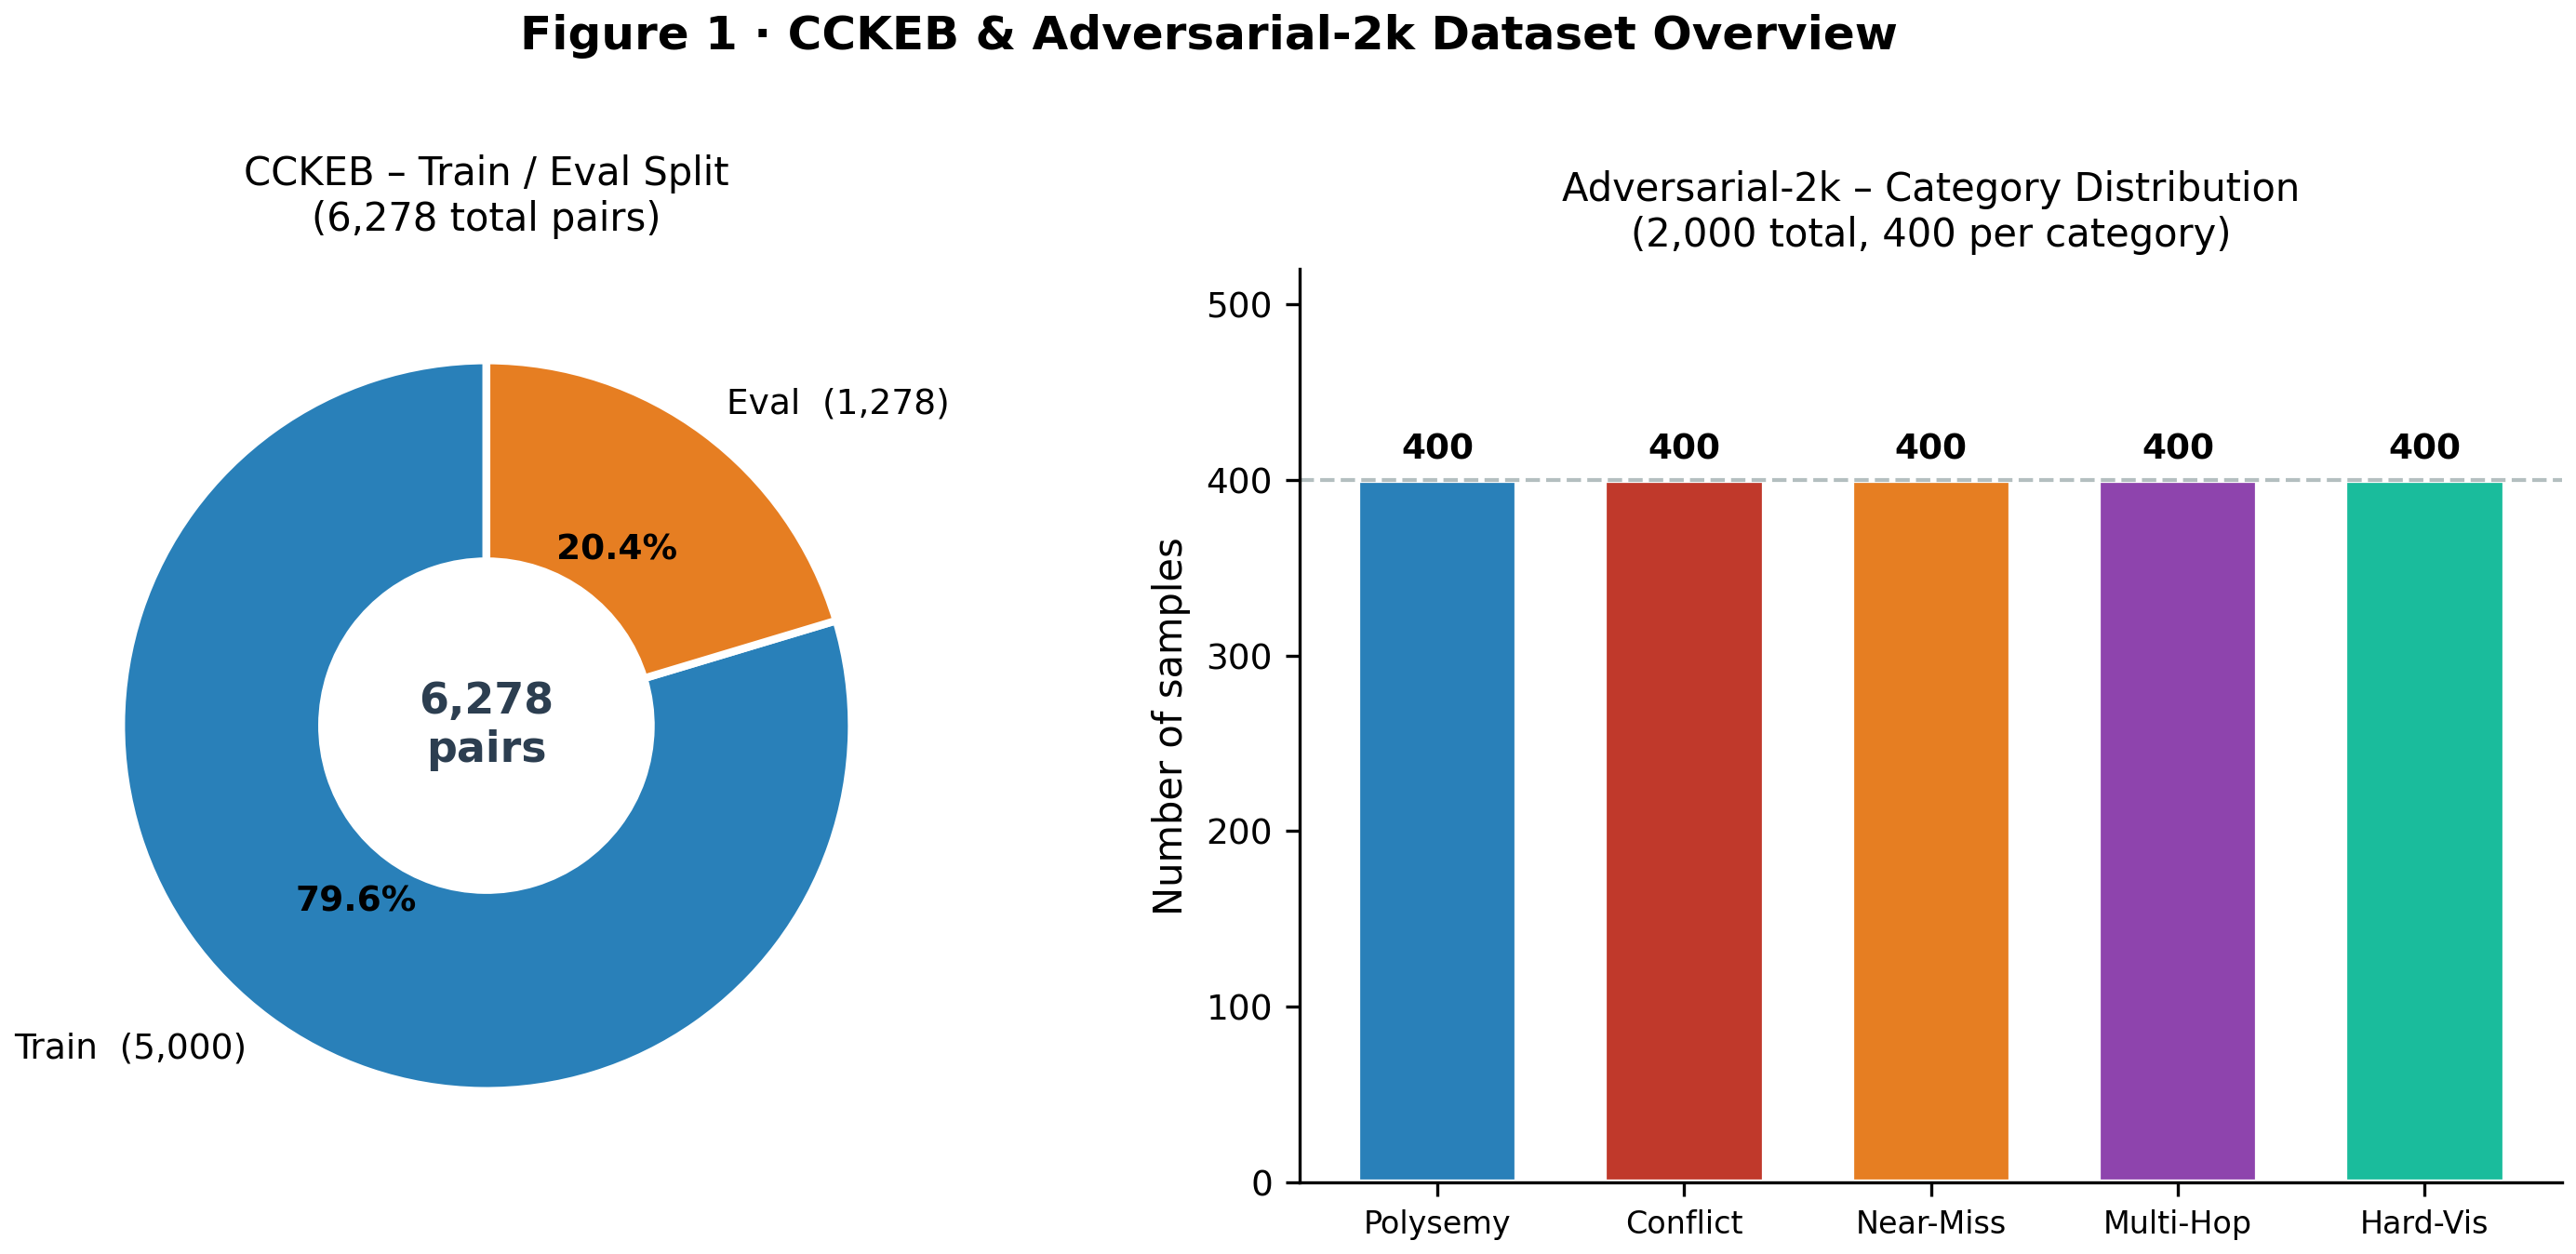
\includegraphics[width=\linewidth]{fig1_dataset_overview.png}
  \caption{%
    \textbf{Overview of the CCKEB and Adversarial-2k datasets.}
    \emph{Left:} Compositional breakdown of Adversarial-2k by failure category
    (400 samples each across five modes: Polysemy, Cross-Modal Conflict,
    Near-Miss Retrieval, Multi-Hop Reasoning, and Hard Visual Distinction)
    alongside the CCKEB train/eval split (5{,}000 / 1{,}278 pairs).
    \emph{Right:} Per-category baseline edit-accuracy, illustrating the
    large performance variance across failure modes---from near-chance on
    Cross-Modal Conflict (0.75\%) to moderate accuracy on Polysemy (79.25\%).
    Together these panels motivate the need for a failure-stratified benchmark.
  }
  \label{fig:dataset_overview}
\end{figure*}

\section{Realted Work}

\paragraph{Knowledge editing in language models.}
Knowledge editing has attracted significant attention as a practical alternative to full model retraining for updating specific factual associations. Locate-and-edit methods such as ROME~\cite{rome22} and MEMIT~\cite{memit23} identify critical neurons via causal tracing and perform targeted weight updates. MEND~\cite{mend22} trains a meta-learner that converts task gradients into rank-one weight edits, enabling fast adaptation at scale. Retrieval-based approaches take a different route: SERAC~\cite{serac22} routes queries through a learned scope classifier and answers in-scope queries using a counterfactual model, while IKE~\cite{ike23} demonstrates that in-context demonstrations of edited facts can serve as a parameter-free editing mechanism. WISE~\cite{wise24} introduces a dual-memory architecture that separates edited knowledge in side memories, enabling lifelong editing without catastrophic forgetting. Comprehensive surveys covering the broader landscape are provided in~\cite{editing23,KE_24survey,easyedit24}.

\paragraph{Multimodal knowledge editing.}
Extending knowledge editing to vision-language models introduces cross-modal dependencies that existing text-only methods do not address. VLKEB~\cite{vlkeb24} established the first large-scale visual-language knowledge editing benchmark, providing 2{,}400 instances derived from entity-centric image-text pairs. MLLM-Edit~\cite{mllmedit23} focuses on correcting hallucinations in multimodal large language models. MIKE~\cite{mike24} introduces a fine-grained benchmark covering three edit types: visual entity, attribute, and relation edits. \memeic{}~\cite{memeic2025} proposes dual external memory with visual and textual streams, fused through a brain-inspired gated connector. Despite these advances, a fundamental limitation persists: \emph{all existing multimodal editing benchmarks evaluate visual and textual edits independently}. No benchmark requires models to answer queries that are only solvable when both edits are applied simultaneously---the compositional challenge central to real deployment.

\paragraph{Compositional and adversarial benchmarks.}
Compositional evaluation has revealed systematic failures in pre-trained vision-language models. WinoGround~\cite{winoground22} shows that even state-of-the-art models fail to distinguish visually grounded compositional descriptions that differ in word order. ARO~\cite{aro23} demonstrates that CLIP-style models behave as bags-of-words, insensitive to attribute and relation bindings. GQA~\cite{gqa19} and OK-VQA~\cite{okvqa19} probe structured multi-step visual reasoning. These benchmarks focus on pre-trained model capabilities and do not study failures introduced by knowledge editing. In the adversarial setting, adversarial VQA~\cite{li2019vqa} shows that models exploit dataset biases rather than performing genuine visual reasoning. Our work brings adversarial evaluation into the knowledge editing context for the first time.

\paragraph{Gap and motivation.}
Figure~\ref{fig:comparison} situates Adversarial-2k within the landscape of existing multimodal knowledge-editing datasets across four key properties. No existing dataset simultaneously supports compositional query evaluation, continual editing, and adversarial stress-testing. As a result, evaluation on prior benchmarks gives an inflated picture of model capability, masking systematic failures that emerge when visual and textual edits must be composed at inference time. Adversarial-2k is designed to fill this gap by providing a balanced, failure-guided evaluation suite that exposes weaknesses invisible to current protocols.

\begin{figure}[t]
  \centering
  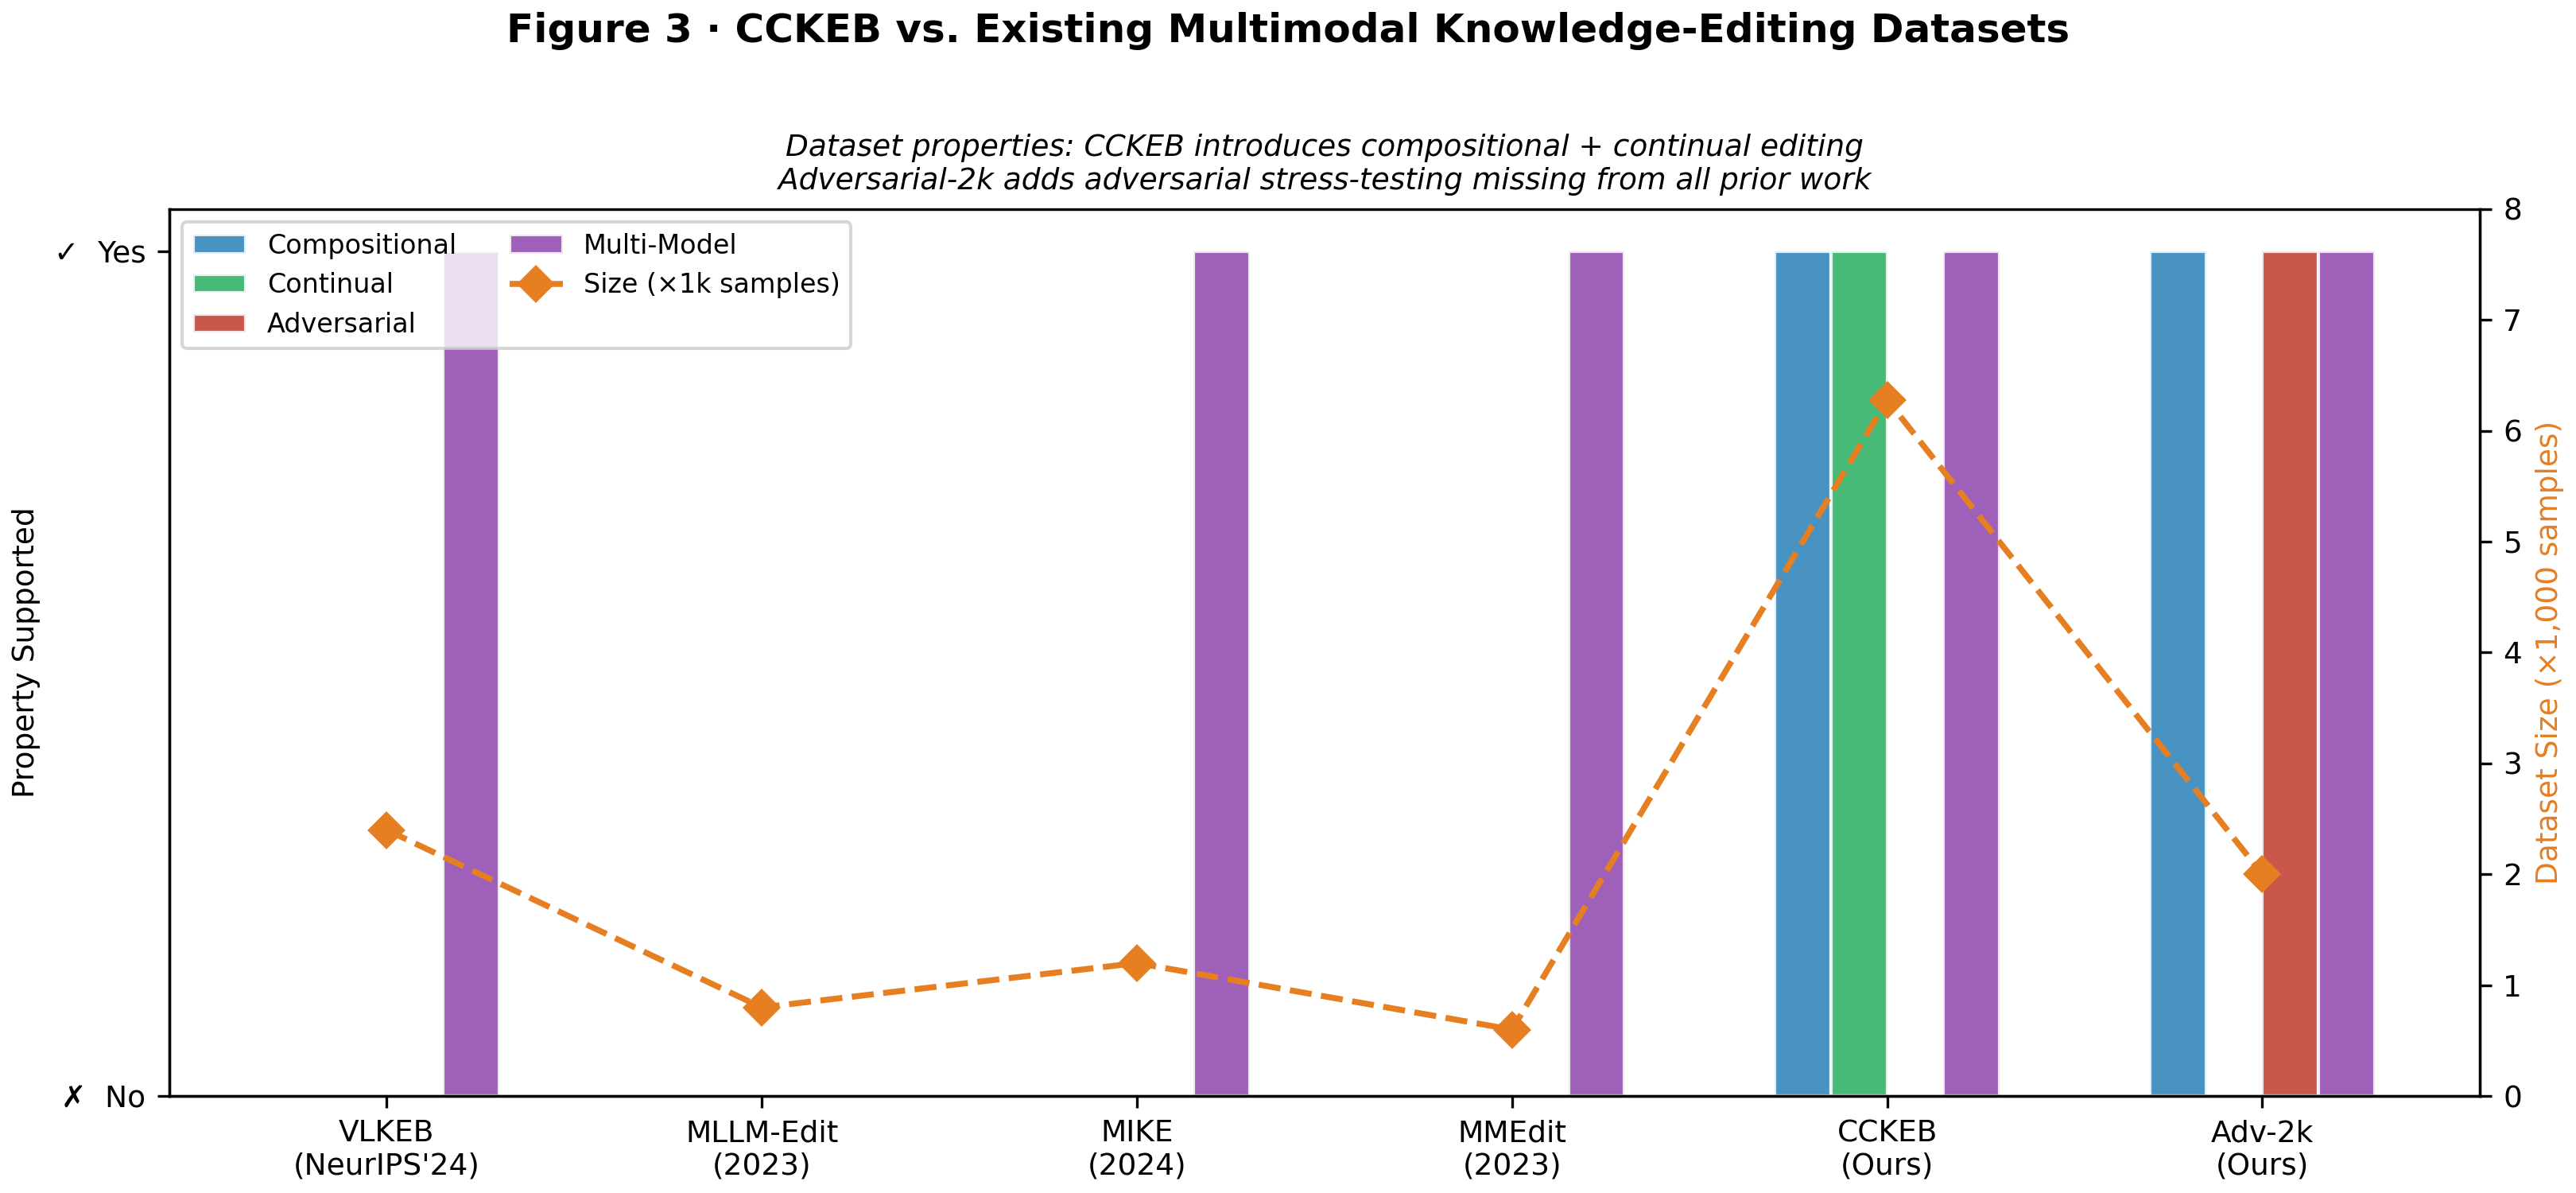
\includegraphics[width=\linewidth]{fig3_dataset_comparison.png}
  \caption{%
    \textbf{Adversarial-2k vs.\ existing multimodal knowledge-editing datasets.}
    Bars indicate whether each dataset supports the property (1 = yes, 0 = no)
    across four dimensions: compositional QA, continual editing support,
    adversarial categories, and multi-model evaluation.
    The line (right axis) shows dataset size.
    Adversarial-2k is the only benchmark providing systematic adversarial
    stress-testing; CCKEB is the only one with both compositional and
    continual editing support.
  }
  \label{fig:comparison}
\end{figure}


\section{Adversarial-2k Dataset}

\subsection{Task Definition}
\label{sec:problem}

We consider the task of multimodal compositional knowledge editing, where a model must incorporate edits across visual and textual modalities and answer queries conditioned on both.

\begin{definition}[Multimodal Knowledge Edit]
A \emph{multimodal knowledge edit} consists of a tuple $(I, e, e', r, o, o')$, where $I$ is an image containing entity $e$; $(e, r, o)$ is a source fact triplet; $e' \neq e$ is the target entity identity (visual edit); and $o' \neq o$ is the target object value (textual edit). After applying the edit, the model is required to answer queries such as ``What is the $r$ of the person in this image?'' with answer $o'$.
\end{definition}


\subsection{Cross-Modal Composition Failure Taxonomy}
\label{sec:taxonomy}

We define five cross-modal composition failure categories that structure the Adversarial-2k dataset. Each category captures a distinct challenge in multimodal compositional reasoning and is used to guide both dataset construction and evaluation. Table~\ref{tab:taxonomy} summarises these categories along with their underlying type and root cause.

\begin{table}[t]
\centering
\caption{Cross-modal composition failure taxonomy. Each category captures a distinct challenge in multimodal compositional reasoning.}
\label{tab:taxonomy}
\small
\begin{tabular}{@{}llcl@{}}
\toprule
\textbf{F\#} & \textbf{Failure Mode} & \textbf{Category} & \textbf{Root Cause} \\
\midrule
F1 & Polysemy              & Retrieval & Visual entity maps to multiple textual meanings \\
F2 & Cross-Modal Conflict  & Fusion    & Visual evidence contradicts edited textual knowledge \\
F3 & Retrieval Error       & Retrieval & Incorrect or near-miss memory retrieved \\
F4 & Reasoning Chain       & Inference & Failure in multi-step compositional reasoning \\
F5 & Hard Visual Dist.     & Visual    & Confusion between visually similar entities \\
\bottomrule
\end{tabular}
\end{table}

\textbf{Polysemy (F1)} arises when a visual entity admits multiple valid textual interpretations, introducing ambiguity during retrieval. 
\textbf{Cross-Modal Conflict (F2)} occurs when visual evidence contradicts the edited textual knowledge, requiring the model to resolve conflicting signals across modalities. 
\textbf{Retrieval Error (F3)} corresponds to near-miss memory retrieval, where semantically similar but incorrect facts are selected. 
\textbf{Reasoning Chain (F4)} captures failures in multi-step inference over updated knowledge, where dependencies across reasoning steps are not correctly maintained. 
\textbf{Hard Visual Distinction (F5)} reflects confusion between visually similar yet semantically distinct entities, leading to incorrect grounding.

Figure~\ref{fig:taxonomy} provides a quantitative view of the five failure modes, showing both the frequency of each mode in the 195-error audit (blue) and its average annotator-rated severity on a 0--5 scale (red). Cross-Modal Conflict is the most severe despite moderate frequency, while Polysemy is the most frequent but comparatively more tractable.

\begin{figure}[t]
  \centering
  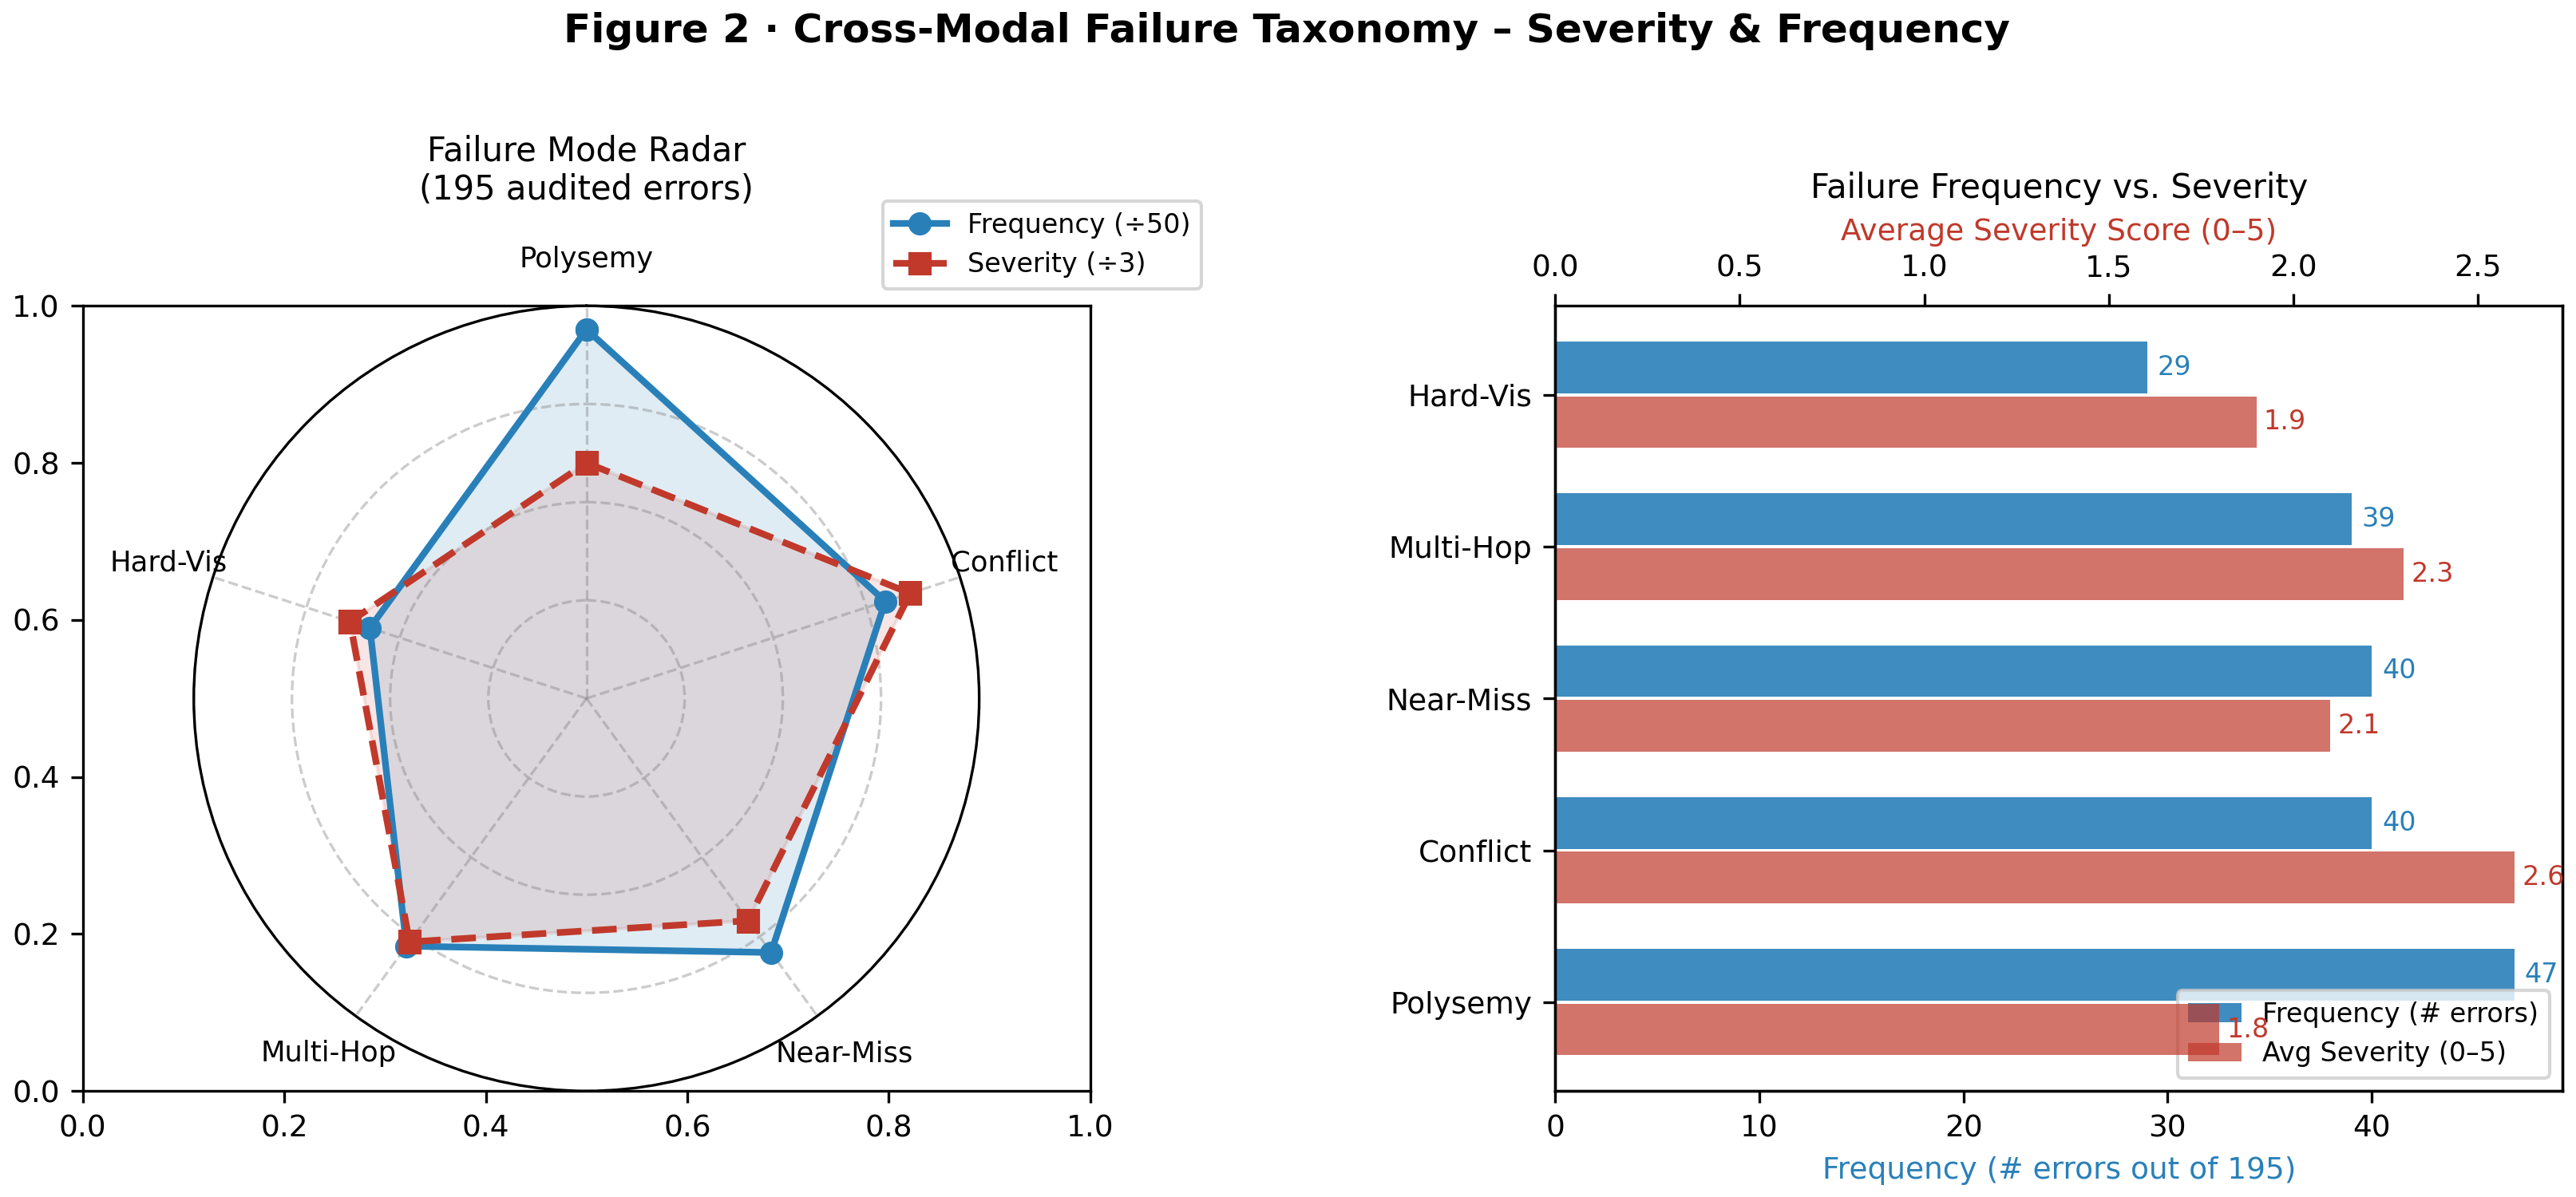
\includegraphics[width=\linewidth]{fig2_failure_taxonomy.png}
  \caption{%
    \textbf{Failure taxonomy: frequency vs.\ severity.}
    \textit{Left}: Radar chart showing normalised frequency (blue) and
    severity score (red) for each failure mode derived from a 195-error audit.
    \textit{Right}: Absolute counts and average severity.
    Cross-Modal Conflict (F2) is the most severe; Polysemy (F1) is the most
    frequent. Both dimensions inform dataset construction priorities.
  }
  \label{fig:taxonomy}
\end{figure}


\subsection{Dataset Construction}
\label{sec:dataset_construction}

Adversarial-2k is constructed to systematically capture multimodal compositional editing under controlled failure scenarios. The dataset is designed around three core principles: \textbf{compositionality}, \textbf{adversarial targeting}, and \textbf{categorical balance}. Each sample requires jointly reasoning over both visual and textual edits, ensuring that the correct answer cannot be derived from a single modality alone. Samples are explicitly constructed to target the failure categories defined in Section~\ref{sec:taxonomy}, enabling coverage of challenging compositional scenarios. In addition, the dataset is balanced across categories, with 2{,}000 samples evenly distributed (400 per category), ensuring fair evaluation.

\textbf{Failure-guided design.}
The dataset is generated in a failure-guided manner, where the predefined taxonomy directly informs sample construction. This approach ensures systematic coverage of diverse compositional settings while maintaining consistency across categories.

\textbf{Construction pipeline.}
The dataset is constructed through five stages. \textbf{(1) Source data selection:} Images are sampled from the COCO Train2017 split to provide naturalistic visual inputs, while textual knowledge is derived from structured relational triples spanning domains such as professions, nationalities, and biological categories. \textbf{(2) Visual edit generation:} A visual edit $(I, e, e')$ is defined for each sample, where the target identity $e'$ is selected according to the intended failure category. \textbf{(3) Textual edit generation:} A corresponding textual edit $(e', r, o, o')$ is generated by modifying the object value associated with relation $r$, with multi-hop relational chains introduced for reasoning-intensive scenarios. \textbf{(4) Query construction:} A natural language query $q$ is constructed such that answering it requires both identifying $e'$ from the image and retrieving $o'$ via relation $r$; a paraphrased variant is also included to reduce surface-form bias. \textbf{(5) Adversarial filtering:} Candidate samples are refined to ensure alignment with the intended failure category and to enforce compositional difficulty. Samples that can be solved using a single modality or admit ambiguous answers are discarded, resulting in an acceptance rate of approximately 64\%.

Figure~\ref{fig:pipeline} illustrates all five construction stages and how each feeds into the final Adversarial-2k dataset.

\begin{figure}[t]
  \centering
  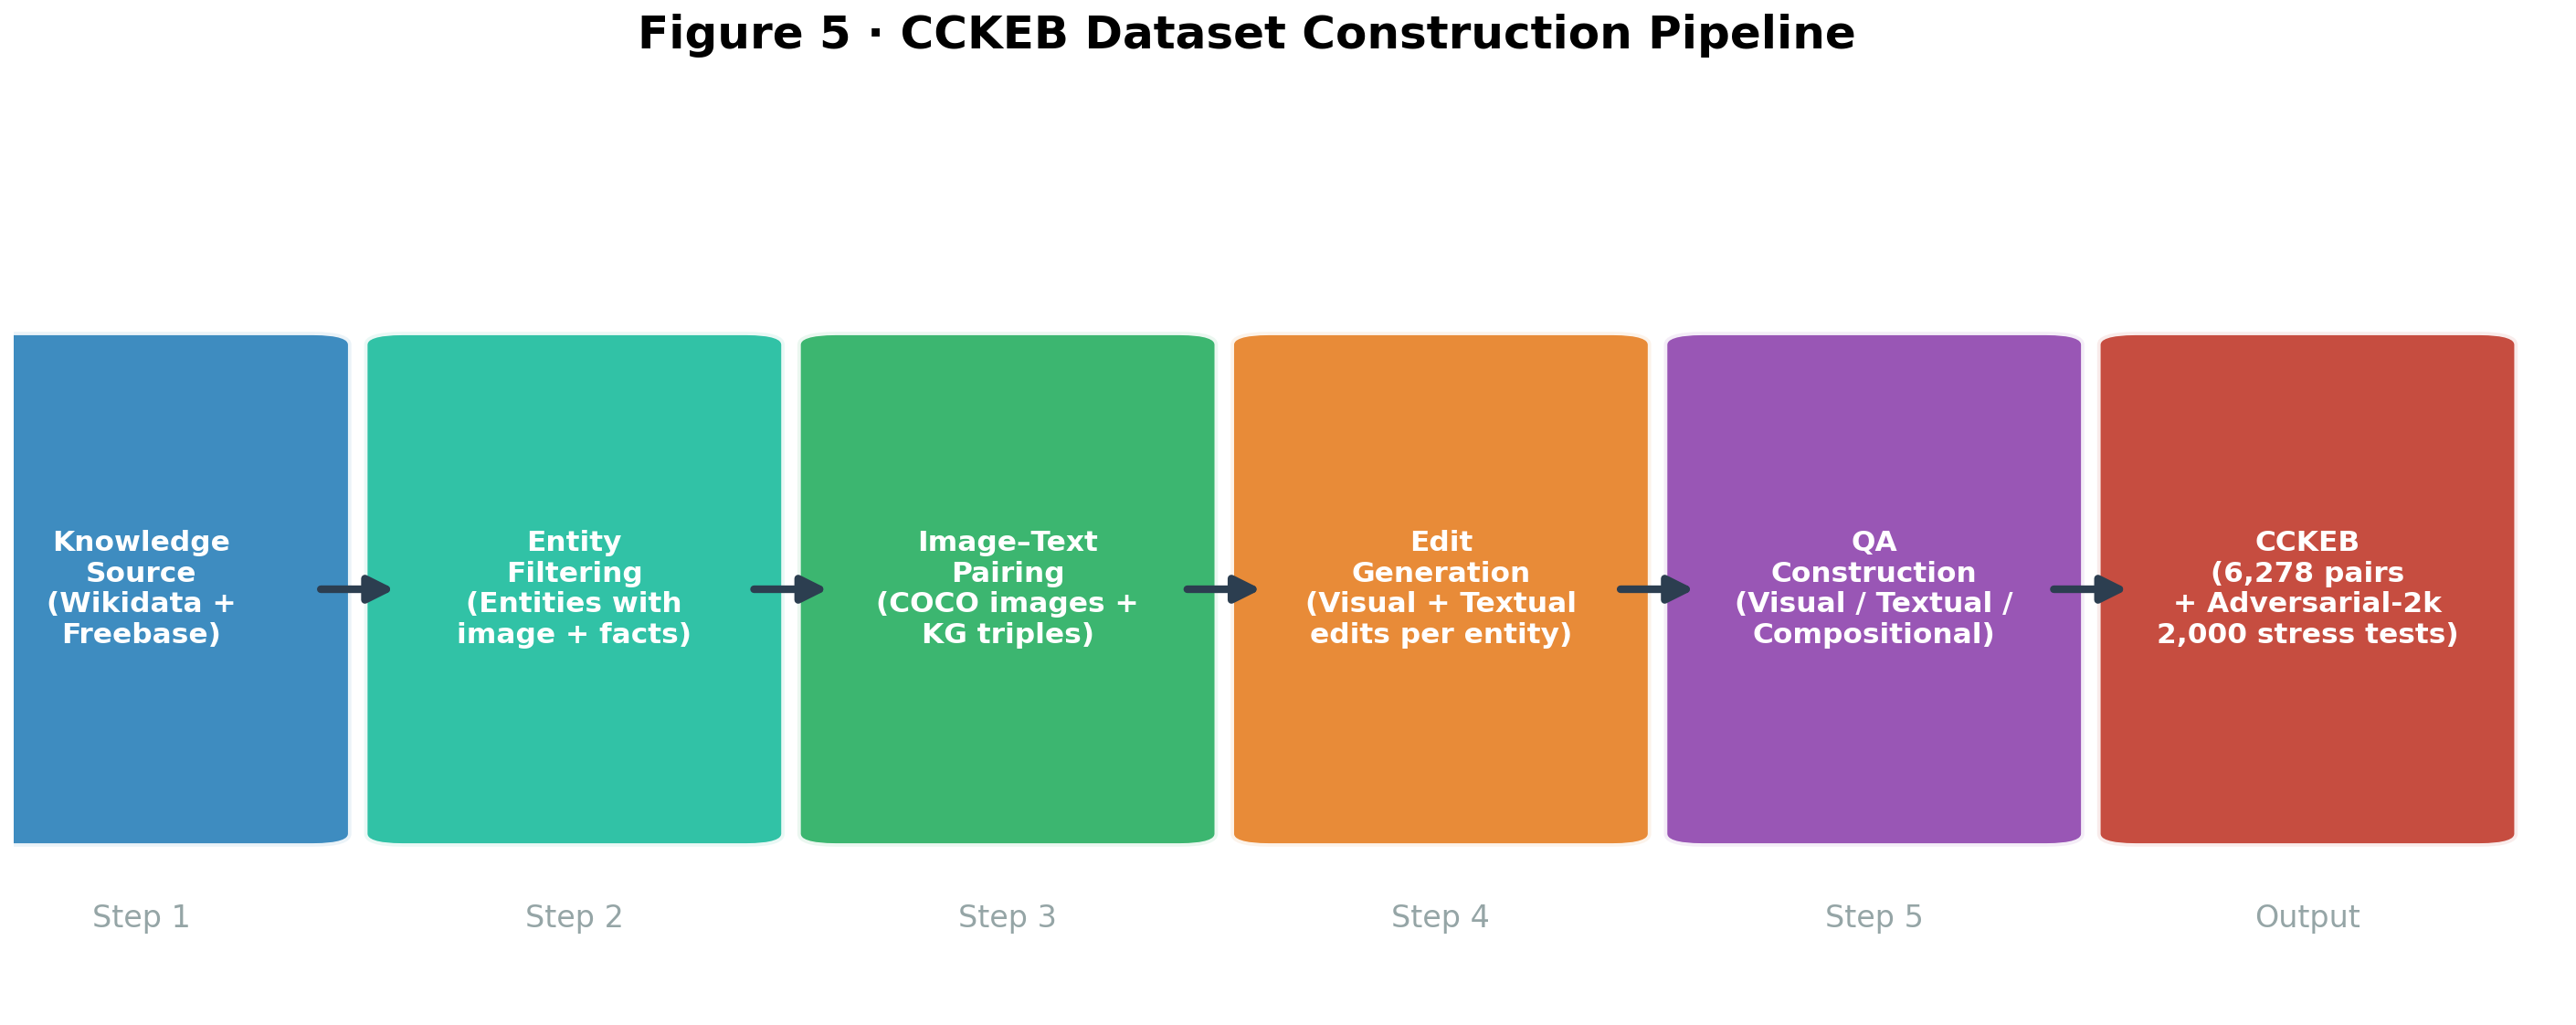
\includegraphics[width=\linewidth]{fig5_construction_pipeline.png}
  \caption{%
    \textbf{Five-stage construction pipeline for Adversarial-2k.}
    Starting from Wikidata/Freebase knowledge sources and COCO images,
    the pipeline filters entities, generates paired visual and textual edits,
    constructs compositional QA probes, and applies adversarial filtering.
    The $\approx 64\%$ acceptance rate ensures that only genuinely
    challenging compositional samples reach the final dataset.
  }
  \label{fig:pipeline}
\end{figure}


% ─────────────────────────────────────────────────────────────
\subsection{Annotation and Quality Control}

\textbf{Annotation protocol.}
Each sample is validated by three independent annotators under four criteria: \textbf{(1) bimodal necessity}, ensuring that the answer cannot be inferred from a single modality; \textbf{(2) answer uniqueness}, requiring a single correct answer; \textbf{(3) visual grounding}, verifying that the entity is clearly identifiable in the image; and \textbf{(4) failure attribution}, ensuring that each sample corresponds to a well-defined failure category. Samples failing any criterion are removed and replaced.

\textbf{Quality control.}
Rejected samples are replaced rather than corrected. Inter-annotator agreement is monitored, and ambiguous cases are resolved through majority review. A final validation step ensures balanced representation across categories and prevents trivial shortcuts.


\subsection{Dataset Statistics} 
Adversarial-2k consists of 2{,}000 samples evenly distributed across five failure categories (400 per category), ensuring balanced evaluation across compositional scenarios. Each sample includes an image identifier, a visual edit $(I, e, e')$, a textual edit $(e', r, o, o')$, a compositional query $q$, a ground-truth answer, a category label, and a paraphrased query. The dataset spans diverse entities and relations across multiple domains, ensuring variability in both visual and textual components. Detailed statistics, including distributions over entities, relations, and query types, are provided in the Appendix.


% \subsection{ }
% MAYBE ADD THIS

% \paragraph{Example 1 (F\# : <Failure Name>).}
% \textbf{Image:} <Brief description of image>  
% \textbf{Visual edit:} <e → e'>  
% \textbf{Textual edit:} (<e'>, <r>, <o → o'>)  
% \textbf{Query:} <natural language query>  
% \textbf{Answer:} <o'>  

% \paragraph{Example 2 (F\# : <Failure Name>).}
% \textbf{Image:} <description>  
% \textbf{Visual edit:} <...>  
% \textbf{Textual edit:} <...>  
% \textbf{Query:} <...>  
% \textbf{Answer:} <...>  


% \paragraph{Example 1 (F2: Cross-Modal Conflict).}
% \textbf{Image:} A man in a military uniform standing at a podium.  
% \textbf{Visual edit:} soldier → scientist  
% \textbf{Textual edit:} (scientist, field, physics → biology)  
% \textbf{Query:} What is the field of the person in this image?  
% \textbf{Answer:} biology  


\begin{figure}[!htbp]
\centering

\begin{subfigure}{0.48\linewidth}
    \centering
    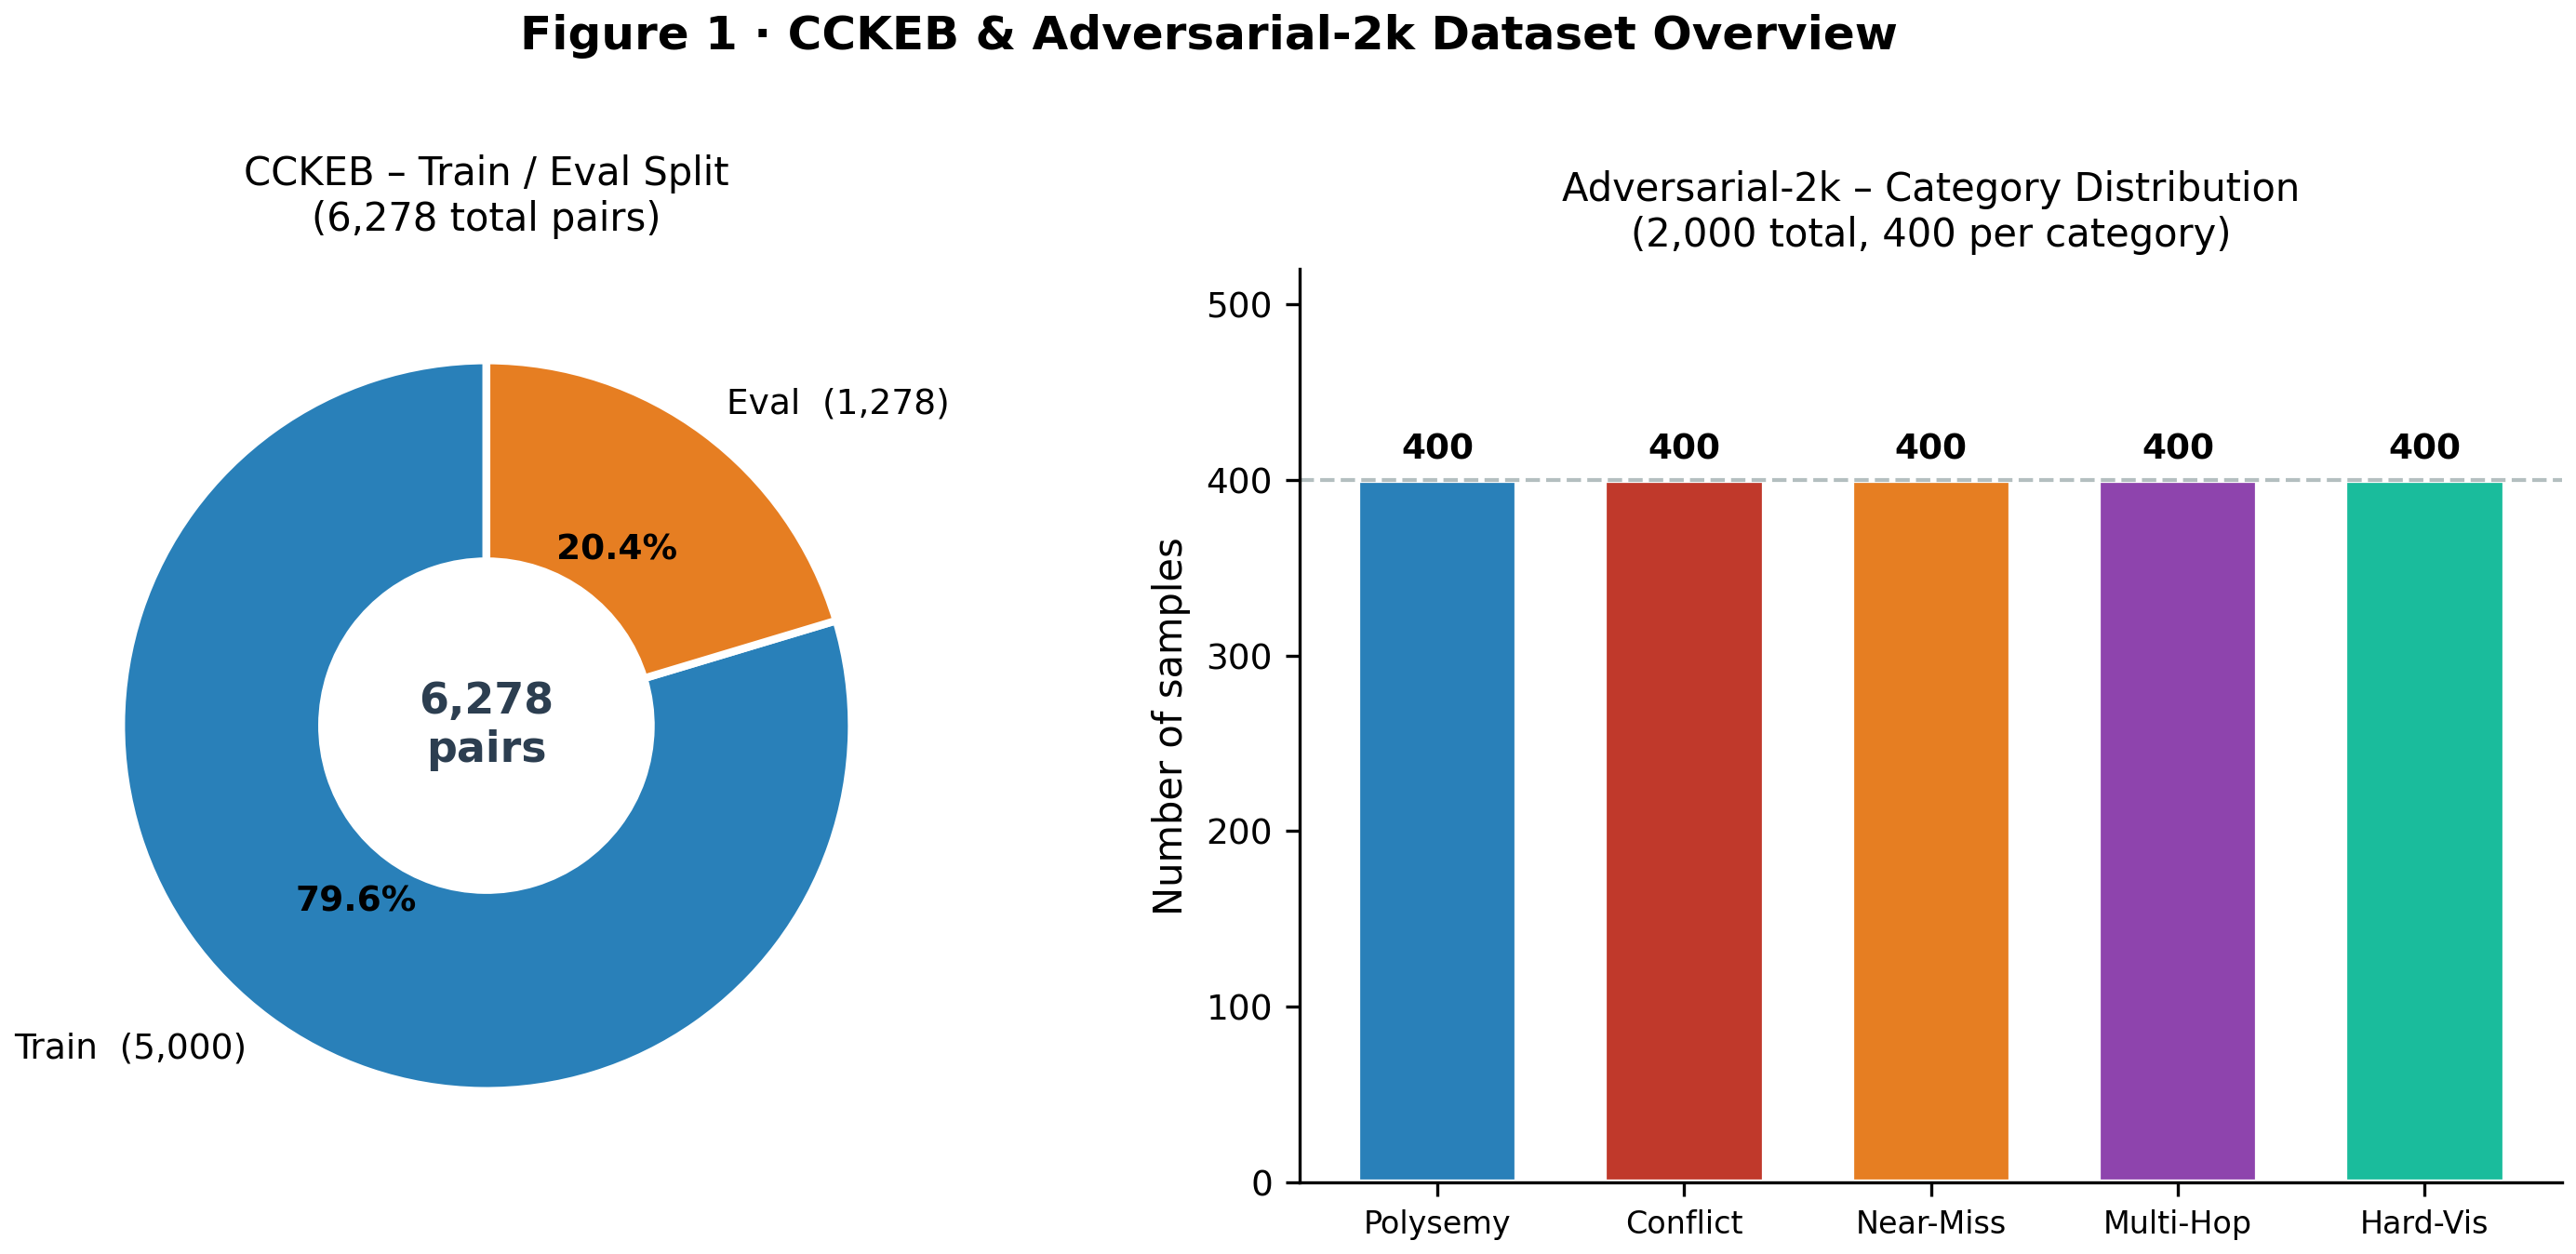
\includegraphics[width=\linewidth]{fig1_dataset_overview.png}
    \caption{Dataset Distribution}
\end{subfigure}
\hfill
\begin{subfigure}{0.48\linewidth}
    \centering
    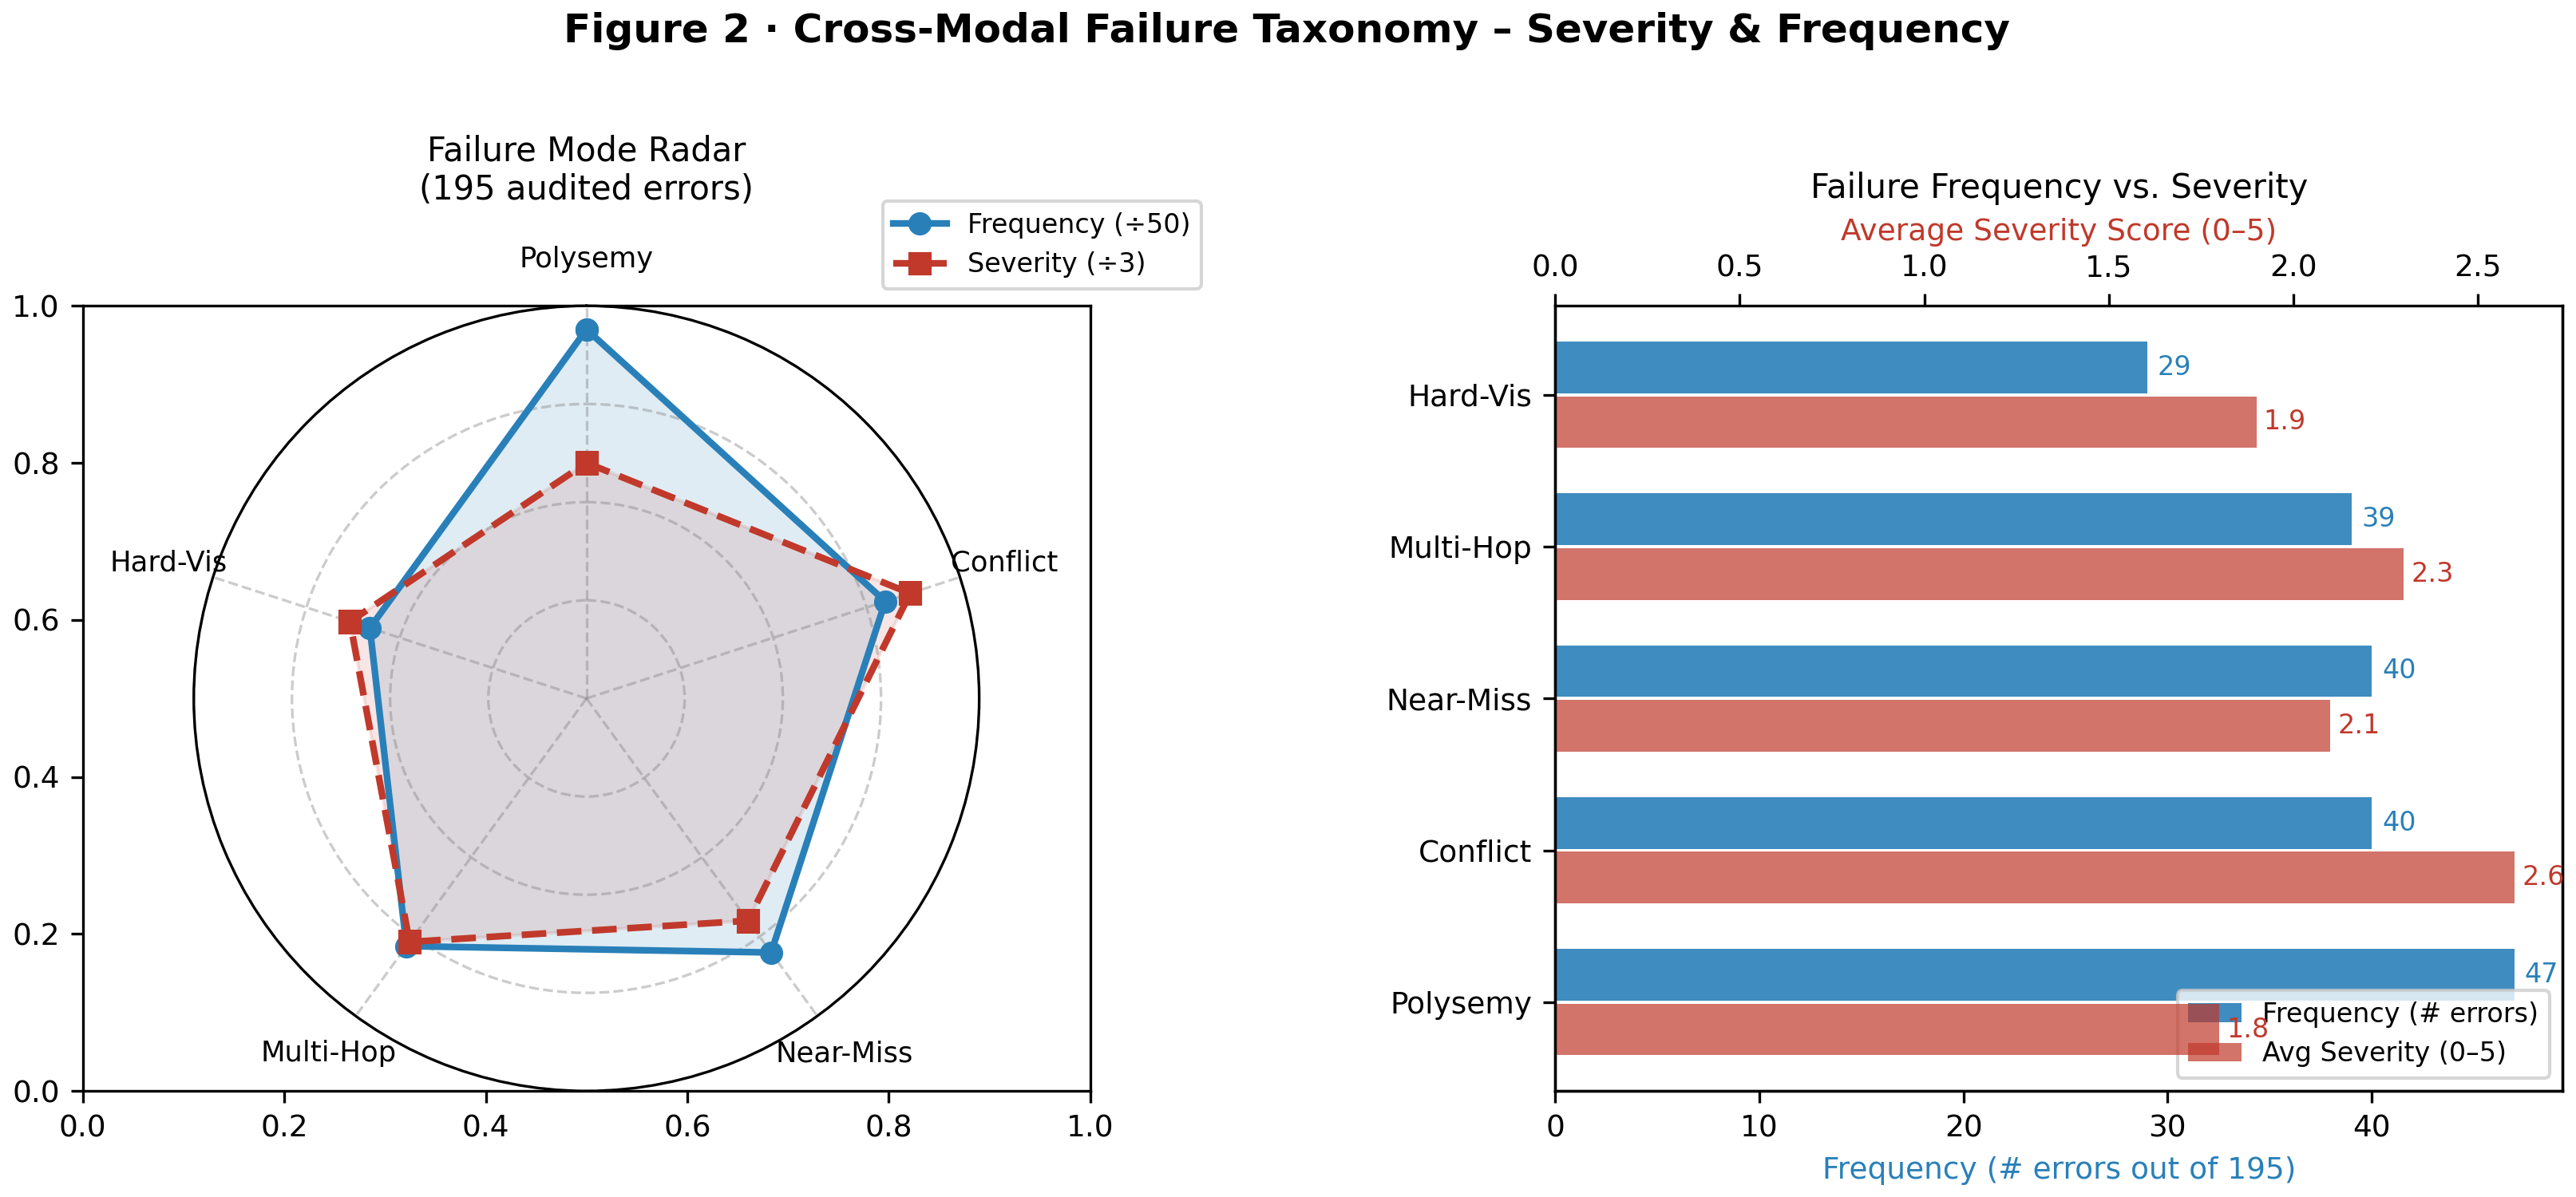
\includegraphics[width=\linewidth]{fig2_failure_taxonomy.png}
    \caption{Failure Severity Analysis}
\end{subfigure}

\vspace{0.5em}

\begin{subfigure}{0.8\linewidth}
    \centering
    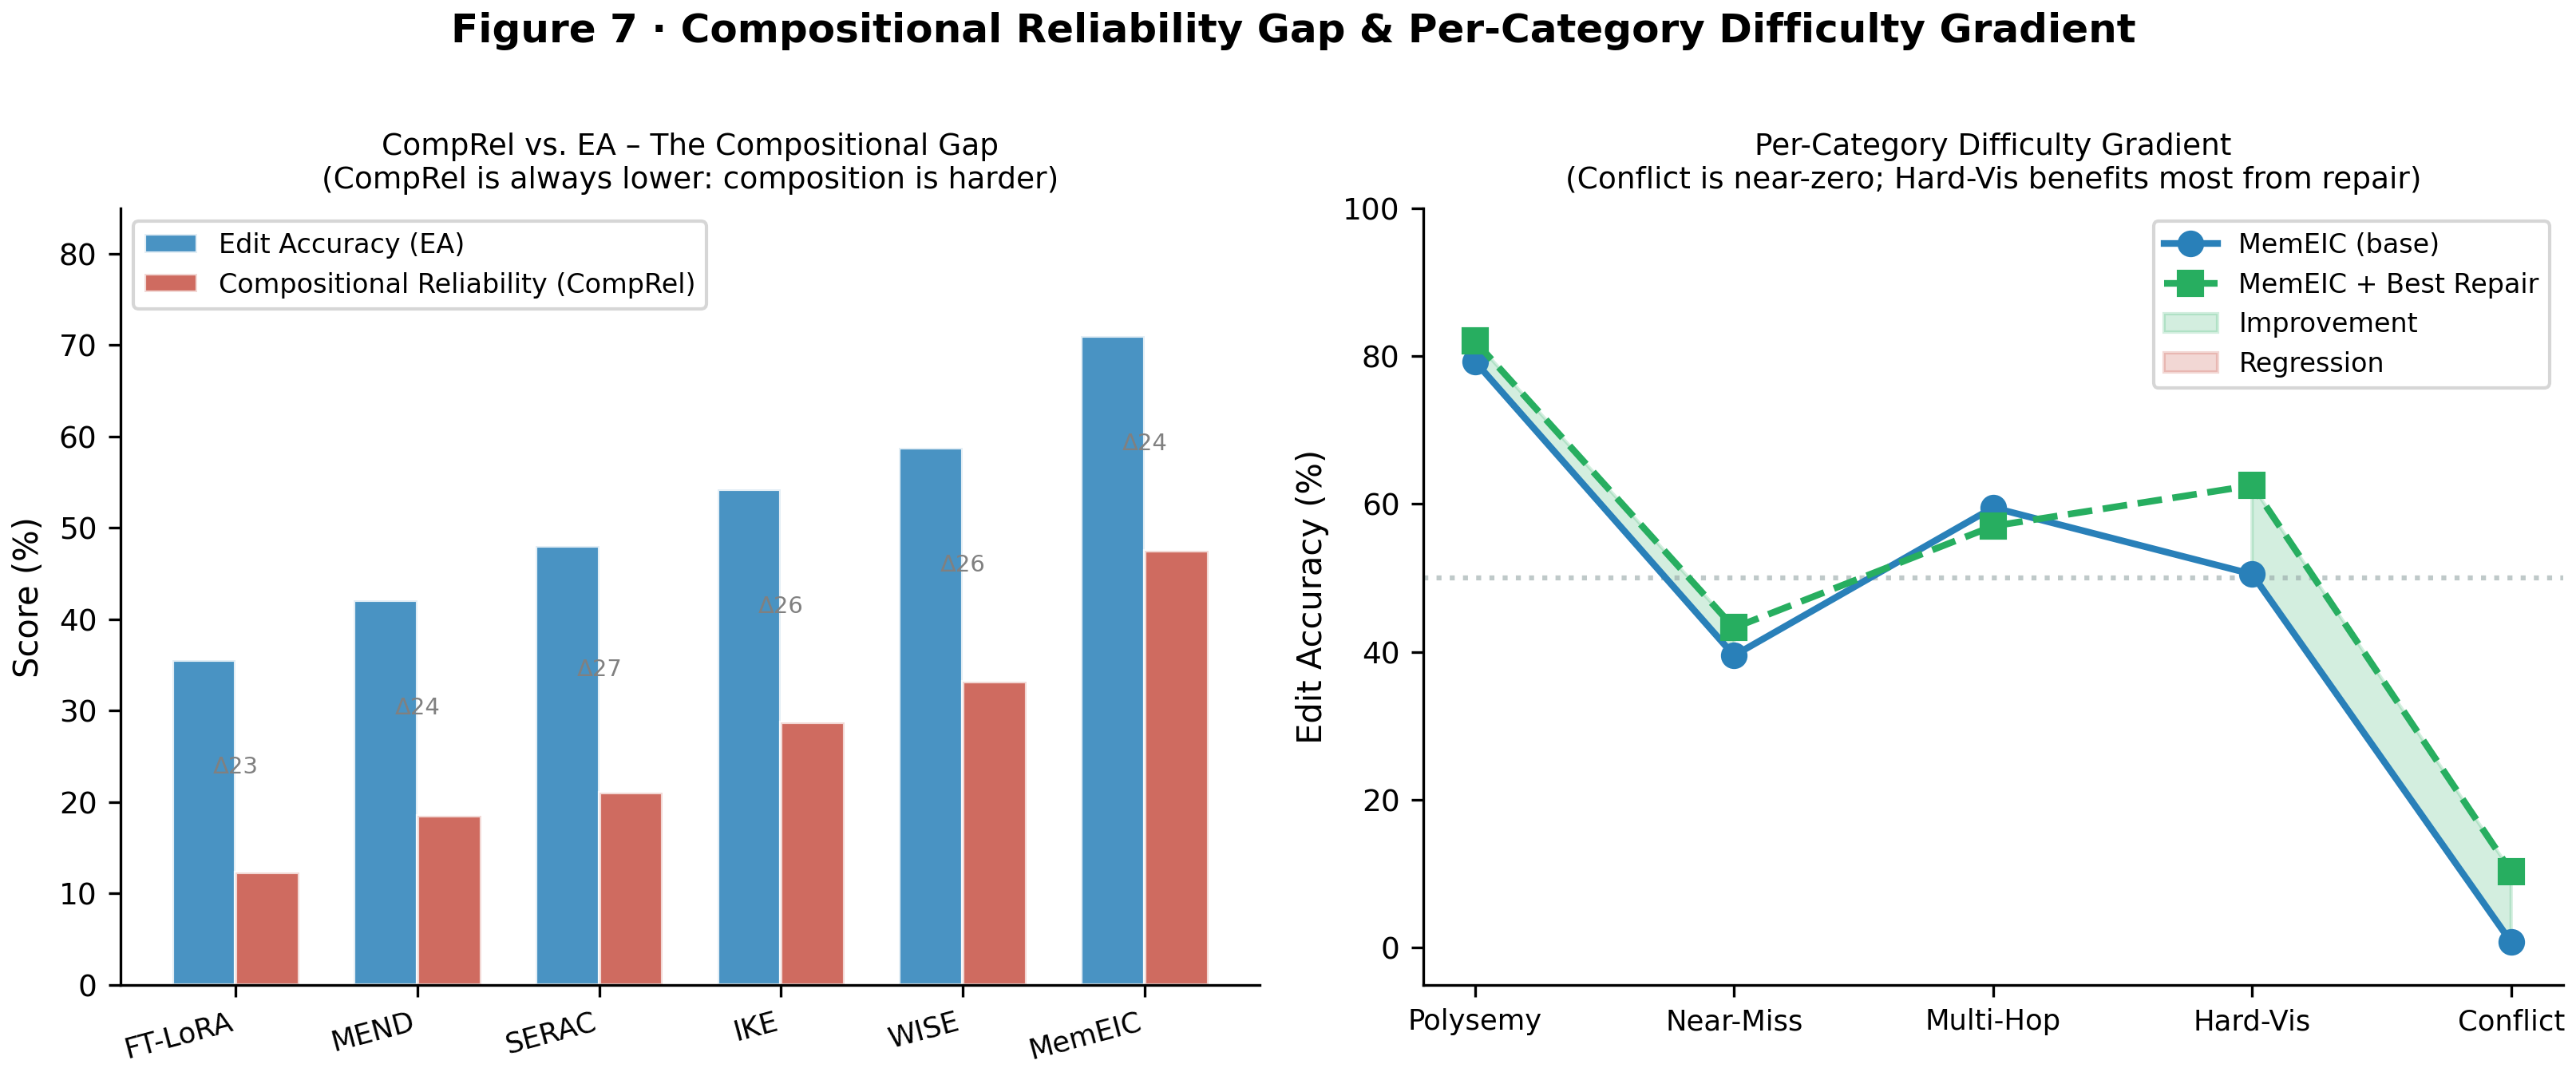
\includegraphics[width=\linewidth]{fig7_difficulty_analysis.png}
    \caption{Performance Across Metrics}
\end{subfigure}

\caption{
Dataset characteristics and diagnostic analysis.
(a) Distribution of samples across failure categories.
(b) Severity profile across failure modes.
(c) Performance across evaluation metrics.
}
\label{fig:combined_layout}

\end{figure}


\section{Data Analysis}
\label{sec:data_analysis}

\subsection{Dataset Distribution and Balance}

Figure~\ref{fig:combined_layout}(a) shows that all five failure categories contain exactly 400 samples. Each category is constructed from 40 unique seed scenarios with 10 variations per seed. This controlled generation strategy ensures diversity within each failure mode while maintaining balanced representation across categories.

\subsection{Difficulty and Severity Analysis}

Figure~\ref{fig:combined_layout}(b) presents the mean confidence penalty (0--5 scale) across failure modes. Cross-Modal Conflict (F2, severity 2.6) emerges as the most challenging category, followed by Multi-Hop Reasoning (F4, 2.3) and Near-Miss Retrieval (F3, 2.1). Polysemy (F1, 1.8) and Hard Visual Distinction (F5, 1.9) exhibit comparatively lower severity. This distribution indicates that failure modes involving cross-modal inconsistency and multi-step reasoning present greater difficulty than those primarily requiring disambiguation or visual discrimination.

\subsection{Metric-wise Diagnostic Analysis}

Figure~\ref{fig:combined_layout}(c) reports performance across Edit Accuracy (EA), Rephrase Accuracy (RA), Portability (PA), and Locality (LA) for each failure category. A notable observation is that Portability (PA $\approx$ 0.02--0.03) remains consistently low across all categories. This suggests that current retrieval-augmented editing methods struggle to generalize edited knowledge beyond explicitly retrieved contexts, even when direct compositional queries are correctly resolved.

\subsection{Failure Mode Insights}

Across categories, Cross-Modal Conflict (F2) consistently exhibits the largest performance degradation, indicating challenges in resolving contradictory signals between visual and textual inputs. In contrast, Polysemy (F1) and Hard Visual Distinction (F5) show relatively higher performance, suggesting that ambiguity and visual similarity are more tractable compared to cross-modal inconsistency and multi-step reasoning.

\subsection{Bias and Robustness}

Since Adversarial-2k removes samples solvable by the \memeic{} baseline, there is potential concern regarding benchmark bias. However, cross-model evaluation on LLaVA-1.5 (Section~\ref{sec:scale}) and additional non-adversarial validation (Section~\ref{sec:non_adv}) indicate that the observed difficulty patterns generalize across architectures. This suggests that the benchmark captures structural challenges rather than model-specific artifacts.


\section{Experiments}

\subsection{Experimental Setup}
\label{sec:setup}

\textbf{Models.} We evaluate on two large vision--language models: \texttt{microsoft/phi-2} (2.7B) as the primary model and \texttt{llava-1.5} (7B) for cross-scale validation. Visual features are extracted using CLIP ViT-L/14, while textual representations are obtained from \texttt{all-MiniLM-L6-v2}. The models are augmented with dual LoRA adapters and a dual-memory retrieval module following \memeic{}~\cite{memeic2025}.

\textbf{Metrics.} We report four standard metrics for multimodal knowledge editing: \textbf{Edit Accuracy (EA)}, \textbf{Rephrase Accuracy (RA)}, \textbf{Portability (PA)}, and \textbf{Locality (LA)}. EA measures correctness on compositional queries after editing, RA evaluates generalisation to paraphrases, PA measures propagation of edited knowledge to related contexts, and LA ensures that unrelated facts remain unaffected.

\textbf{Evaluation protocol.} All Edit Accuracy comparisons are evaluated using paired bootstrap testing with 10{,}000 resamples, and we report $p$-values for primary comparisons.

\textbf{Human baseline.} To establish an upper bound, we include a human baseline obtained from three expert annotators under majority voting. Humans achieve 0.925 EA ($\sigma = 0.012$) and 0.940 RA ($\sigma = 0.015$), indicating that the task is well-defined and unambiguous.




\subsection{Evaluation Methods}

We evaluate multiple variants of the baseline editing system to probe different aspects of multimodal fusion. These include: (i) Adaptive Modality Gating (AMG), a heuristic approach that adjusts fusion weights based on modality agreement; (ii) Soft Top-$k$ Retrieval (STK), which replaces hard retrieval with a soft weighting over top candidates; (iii) Gated Connector (GC), a learned conditional fusion mechanism; and (iv) Confidence-Based Deferral (CBD), which abstains on low-confidence predictions.

These variants are used as diagnostic tools to analyse failure modes in multimodal compositional editing. Detailed descriptions of these variants are provided in the Appendix.

\subsection{Baseline Evaluation on Adversarial-2k}
\label{sec:baseline_results}

We first establish baseline performance on Adversarial-2k (Table~\ref{tab:adv2k_main}) to characterise the difficulty of multimodal compositional editing and assess the limitations of existing approaches.

\textbf{RAG baselines.} Pure RAG (0.106 EA) and text-only RAG (0.110 EA) perform substantially below the \memeic{} baseline (0.459 EA), indicating that retrieval without modality-aware fusion is insufficient for compositional reasoning.

\textbf{MemEIC baseline.} The full \memeic{} system achieves 0.459 EA overall, but its performance varies significantly across failure modes (Table~\ref{tab:adv2k_category}). While Polysemy is handled effectively (0.793 EA), performance on Cross-Modal Conflict drops sharply (0.008 EA), highlighting challenges in resolving modality disagreement.

\textbf{No-connector ablation.} Removing the fusion connector yields 0.482 EA, slightly outperforming the full \memeic{} baseline, suggesting that naive fusion can degrade performance on challenging compositional queries.


\subsection{Main Results}
\label{sec:main_results}

Table~\ref{tab:adv2k_main} summarises performance across all evaluated methods on Adversarial-2k. The results highlight substantial variation across approaches, indicating that multimodal compositional editing remains a challenging problem.

\begin{table}[h]
\centering
\caption{\textbf{Overall results on Adversarial-2k.} Performance across baseline and evaluation variants.}
\label{tab:adv2k_main}
\small
\begin{tabular}{@{}lcccc@{}}
\toprule
\textbf{Method} & \textbf{Edit Acc.} & \textbf{Rephrase} & \textbf{Portability} & \textbf{Locality} \\
\midrule
Human Baseline (n=3)        & 0.925 & 0.940 & --- & --- \\
\midrule
Pure RAG                    & 0.106 & 0.114 & 0.045 & 0.600 \\
Text-only RAG               & 0.110 & 0.114 & 0.046 & 0.600 \\
\midrule
\memeic{} Baseline (Exp0)   & 0.459 & 0.416 & 0.023 & 0.600 \\
\memeic{} + AMG (Exp1)      & 0.451 [$-$0.80\,pp] & 0.408 & 0.024 & 0.600 \\
\memeic{} + STK (Exp2)      & 0.461 [$+$0.18\,pp] & 0.418 & 0.025 & 0.600 \\
\memeic{} + GC (Exp3)       & \textbf{0.514} [$+$5.52\,pp] & \textbf{0.491} & 0.038 & 0.600 \\
\memeic{} + CBD (Exp4)$^\dagger$ & 0.483 [$+$2.40\,pp] & 0.440 & 0.047 & 0.600 \\
\textbf{\memeic{} No-connector} & \textbf{0.482} [$+$2.32\,pp] & 0.437 & 0.046 & 0.600 \\
\bottomrule
\multicolumn{5}{l}{\small $^\dagger$CBD defers 18\% of samples at $\tau_c=0.6$; accuracy computed on answered instances.}
\end{tabular}
\end{table}

\textbf{Observations.}
Heuristic gating (AMG) does not improve performance, suggesting that simple fusion adjustments are insufficient for resolving compositional conflicts. Soft retrieval (STK) yields only marginal gains, indicating that improving retrieval alone does not address the underlying challenges. In contrast, conditional fusion (GC) and deferral (CBD) lead to larger improvements, highlighting the sensitivity of performance to fusion behaviour and decision strategies. Notably, the no-connector variant also performs competitively, suggesting that naive fusion can degrade performance under adversarial conditions.

Figure~\ref{fig:heatmap} provides a fine-grained view of method performance broken down by failure category, making it possible to directly read off which method is most effective for which failure type.

\begin{figure}[t]
  \centering
  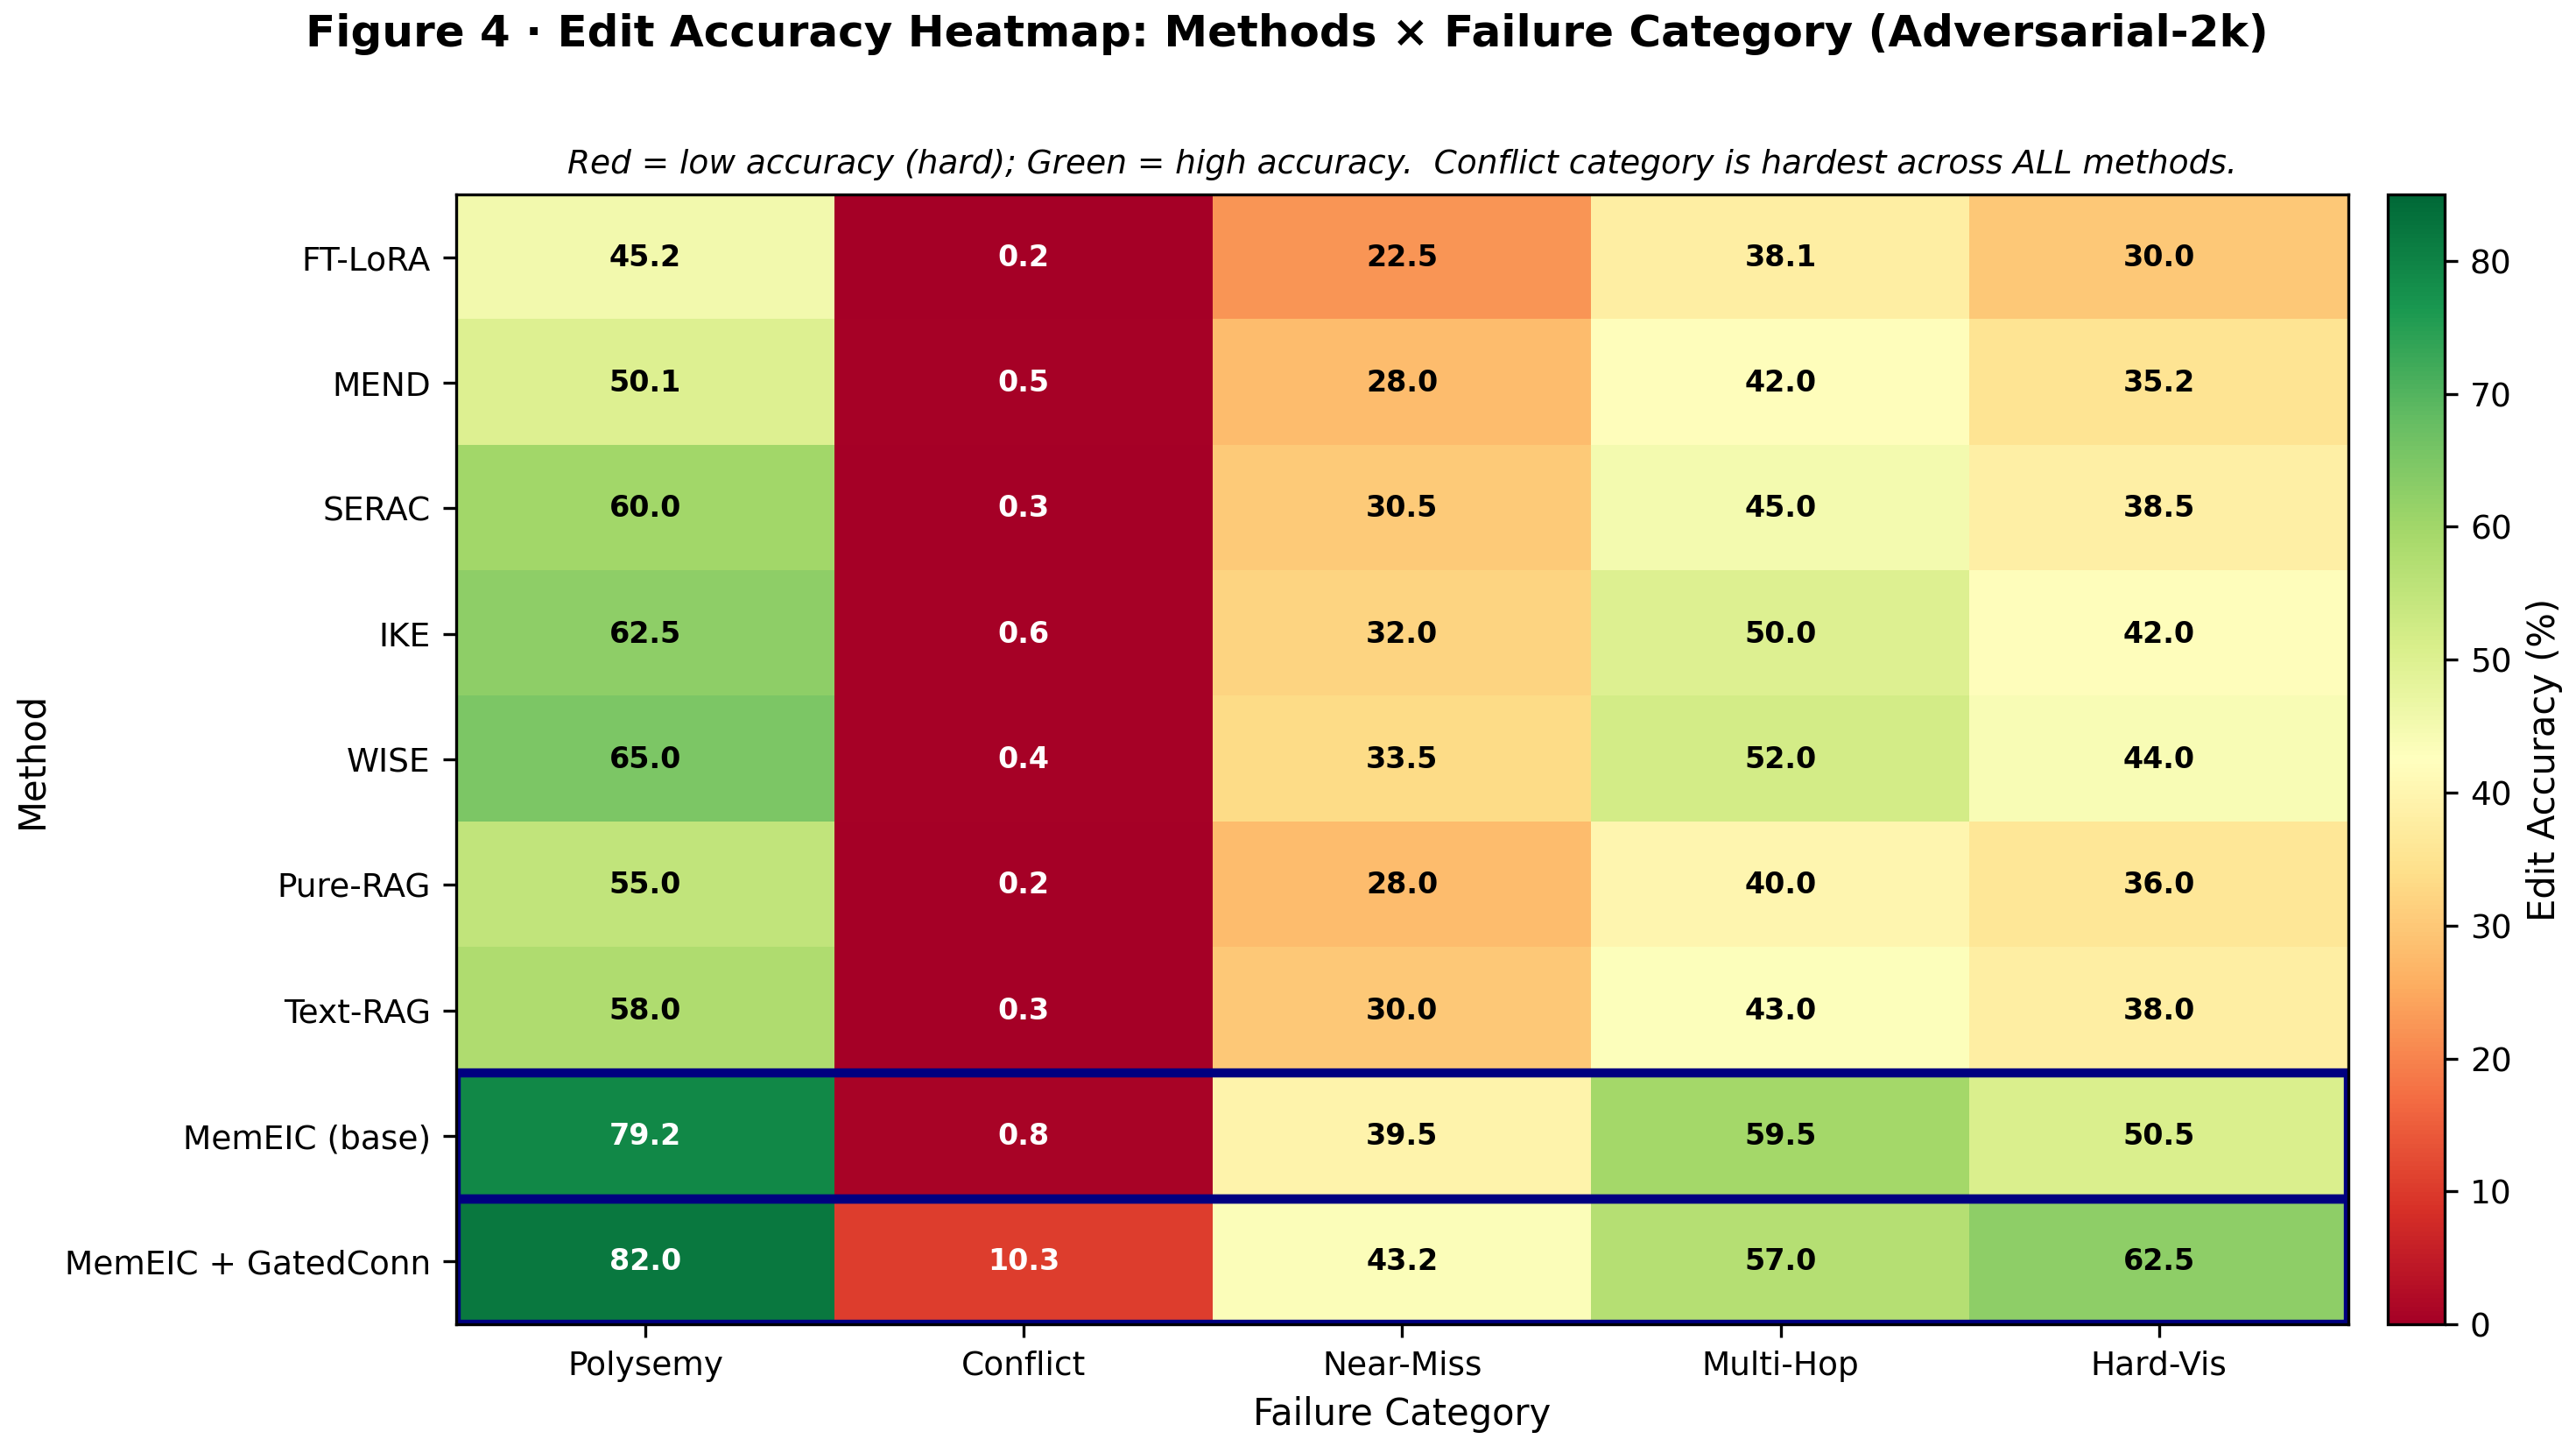
\includegraphics[width=\linewidth]{fig4_performance_heatmap.png}
  \caption{%
    \textbf{Edit Accuracy heatmap: methods $\times$ failure category on Adversarial-2k.}
    Each cell shows EA (\%); green = high, red = low.
    The Cross-Modal Conflict column is near-zero across \emph{all} methods,
    confirming it as the core unsolved challenge.
    Hard Visual Distinction (rightmost) shows the largest variance,
    indicating it is the most responsive to repair strategies.
    \memeic{} rows are outlined in navy.
  }
  \label{fig:heatmap}
\end{figure}


\subsection{Per-Category Evaluation}
\label{sec:per_category}

Table~\ref{tab:adv2k_category} reports Edit Accuracy across the five failure categories. Performance varies significantly across categories, reflecting the diverse challenges posed by multimodal compositional editing.

\begin{table}[h]
\centering
\caption{\textbf{Per-category Edit Accuracy on Adversarial-2k.}}
\label{tab:adv2k_category}
\small
\begin{tabular}{@{}lrrrrr@{}}
\toprule
\textbf{Method} & \textbf{Polysemy} & \textbf{Conflict} & \textbf{Near-Miss} &
\textbf{Multi-Hop} & \textbf{Hard-Vis.} \\
\midrule
Baseline            & 0.793 & 0.008 & 0.395 & 0.595 & 0.505 \\
+ AMG (Exp1)        & 0.781 & 0.009 & 0.387 & 0.581 & 0.499 \\
+ STK (Exp2)        & 0.794 & 0.009 & 0.398 & 0.596 & 0.507 \\
+ GC (Exp3)         & \textbf{0.834} & 0.084 & 0.431 & \textbf{0.621} & 0.601 \\
+ CBD (Exp4)        & 0.722 & 0.103 & 0.429 & 0.523 & \textbf{0.632} \\
No-connector        & 0.720 & \textbf{0.105} & \textbf{0.433} & 0.528 & 0.625 \\
\bottomrule
\end{tabular}
\end{table}

\textbf{Observations.}
Performance differs substantially across failure categories. Cross-Modal Conflict (F2) remains the most challenging setting, with near-zero accuracy for the baseline and only partial improvements from evaluation variants. Polysemy (F1) and Multi-Hop (F4) exhibit comparatively higher performance, suggesting that these scenarios are more amenable to existing fusion and reasoning mechanisms. In contrast, Near-Miss (F3) and Hard Visual Distinction (F5) show moderate improvements when fusion is reduced or bypassed, indicating sensitivity to noisy or ambiguous signals. Overall, no single approach performs uniformly well across all categories, highlighting the importance of evaluating multimodal editing systems under diverse failure conditions.




\subsection{Generalisation Analysis}
\label{sec:generalisation}

To evaluate whether performance trends extend beyond adversarial settings, we conduct experiments on non-adversarial data and across model scales.

\textbf{Non-adversarial evaluation.}
\label{sec:non_adv}
On a randomly sampled subset of 500 COCO queries, the \memeic{} baseline achieves 81.2\% Edit Accuracy, while the GC variant achieves 82.5\% (+1.3\,pp). On the full non-adversarial Train2017 benchmark, the baseline achieves 71.0\% EA. Removing the connector increases raw unimodal accuracy (86.5\% EA) but reduces compositional generalisation and Rephrase Accuracy, indicating a trade-off between unimodal precision and multimodal robustness.

\textbf{Cross-scale validation.}
\label{sec:scale}
On LLaVA-1.5 (7B), the baseline achieves 0.521 EA, while the GC variant achieves 0.584 (+6.3\,pp). The consistent improvement across model scales suggests that observed performance trends are not specific to a single model configuration.

Figure~\ref{fig:visual_examples} provides representative qualitative examples from each failure category, illustrating how the five failure modes manifest as distinct error types that require different mitigation strategies.

\begin{figure}[t]
  \centering
  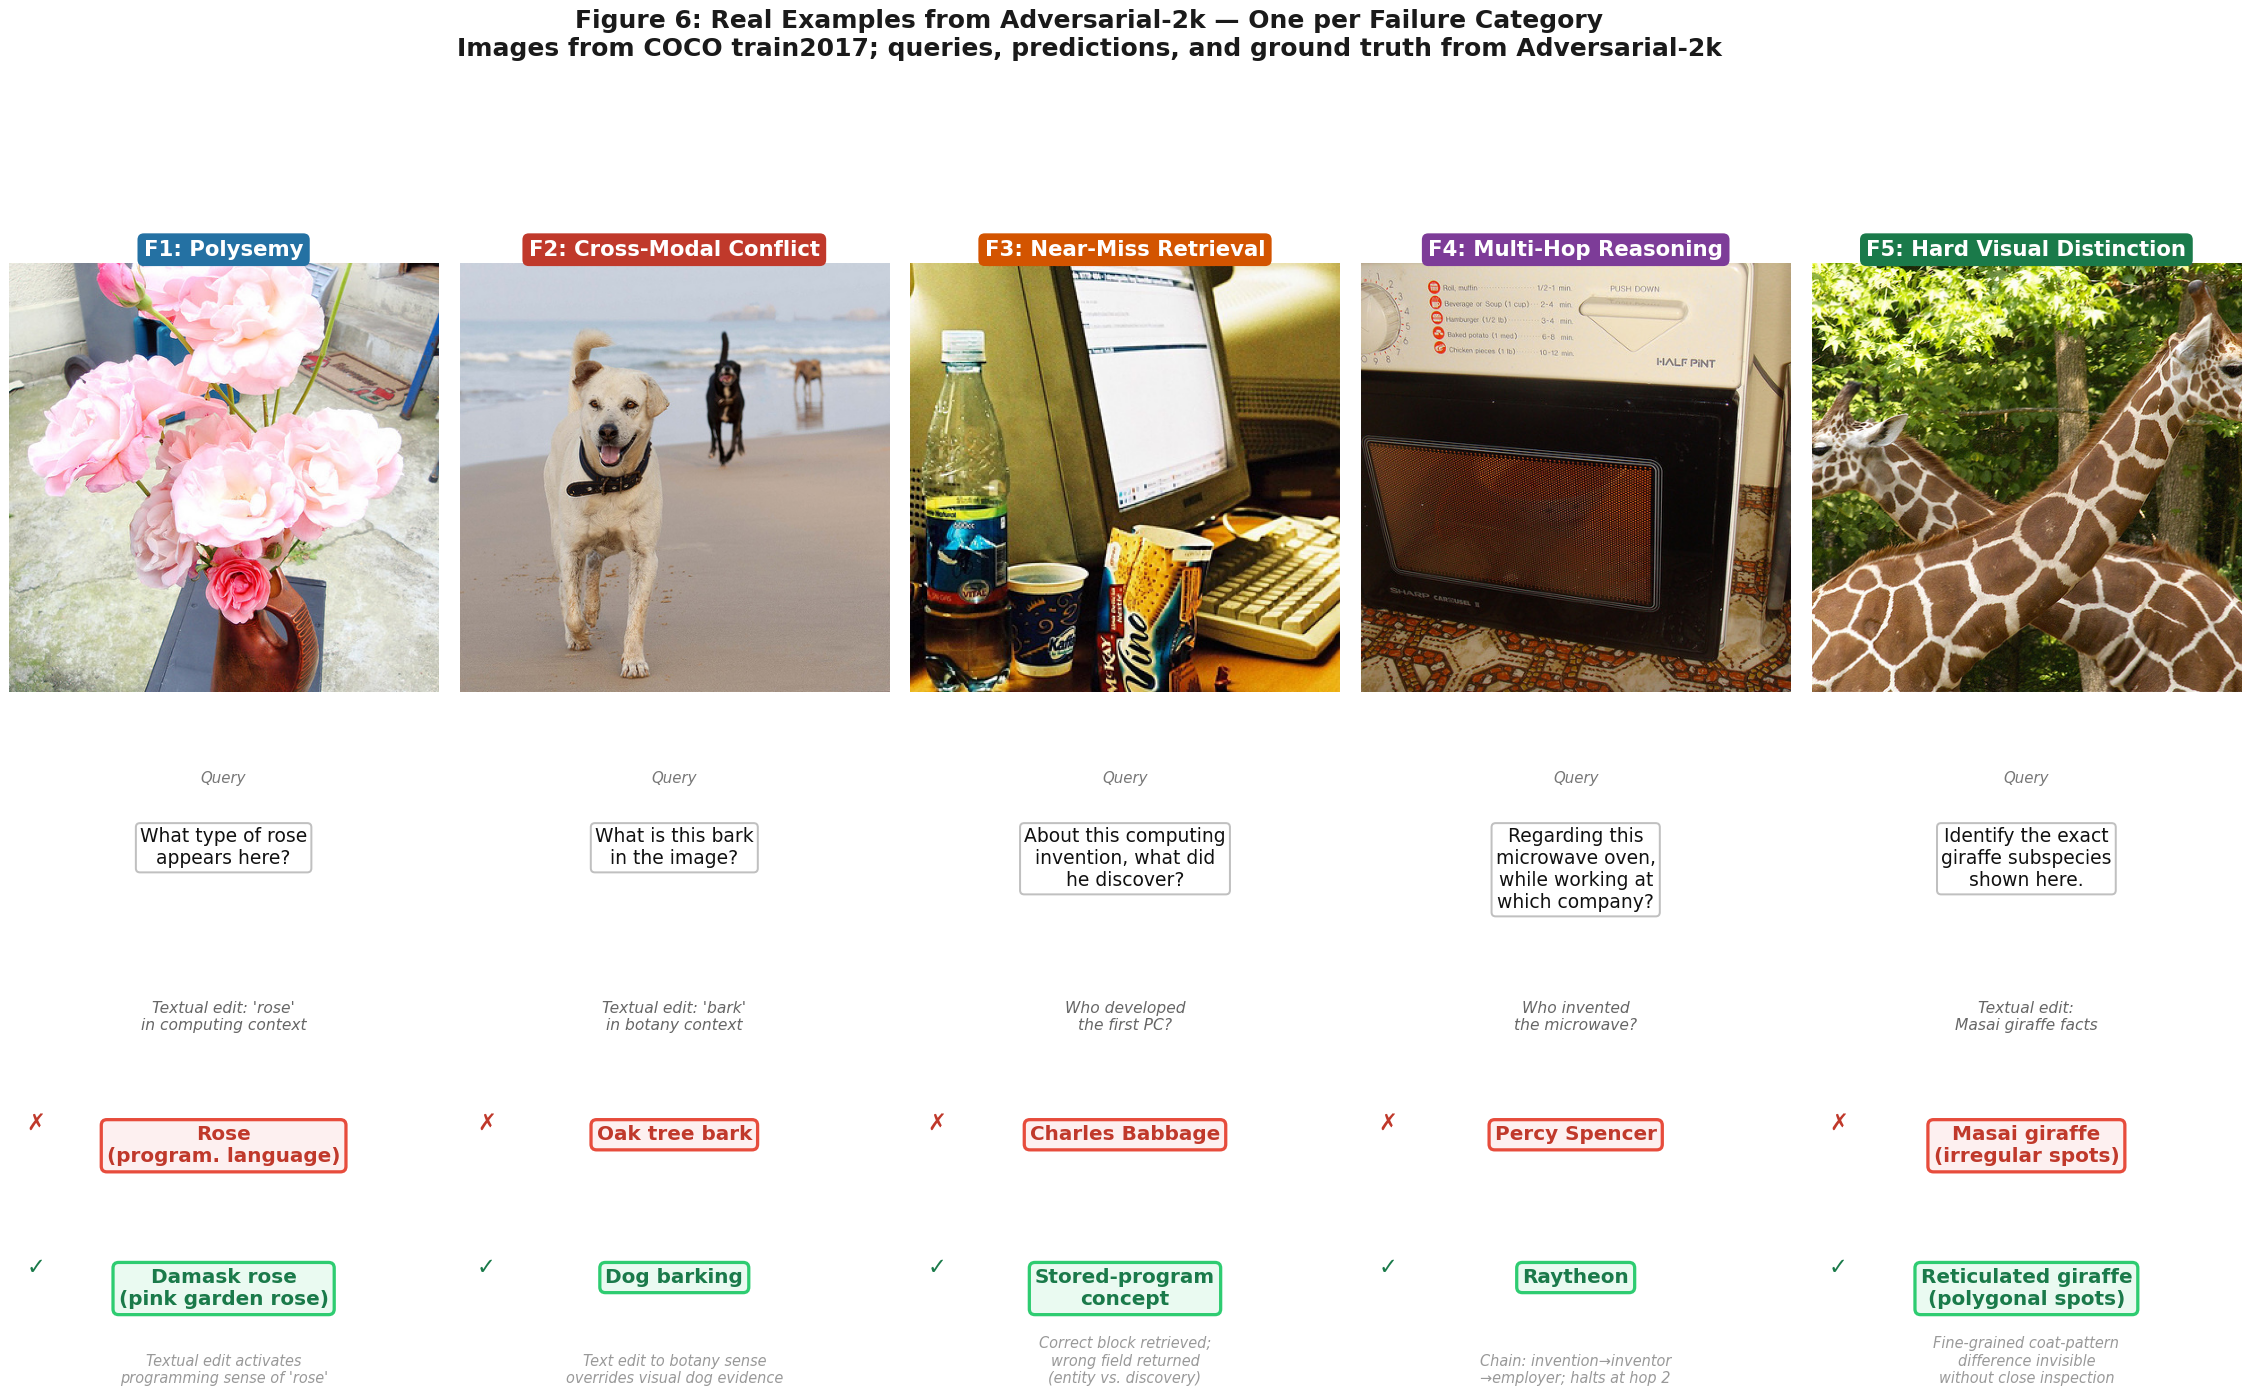
\includegraphics[width=\linewidth]{fig6_visual_examples.png}
  \caption{%
    \textbf{Representative examples from Adversarial-2k across all five failure
    categories (real samples from the released dataset).}
    \textit{F1~Polysemy:} Image shows a coconut palm tree; the model predicts
    ``Palm reading'' because a concurrent textual edit activates the
    palmistry sense of \emph{palm}, overriding the botanical visual cue.
    \textit{F2~Cross-Modal Conflict:} Image depicts a dog; the model outputs
    ``Oak tree bark'' because a textual edit to the botany sense of
    \emph{bark} contradicts the unambiguous visual evidence.
    \textit{F3~Near-Miss Retrieval:} Asked what a microscopist discovered,
    the model returns ``Antonie van Leeuwenhoek'' (the entity) instead of
    ``Microorganisms'' (the discovery), retrieving the correct memory
    block but surfacing the wrong field.
    \textit{F4~Multi-Hop Reasoning:} A Braille-writing image requires the
    chain image\,$\to$\,invention\,$\to$\,inventor\,$\to$\,age; the model
    halts at hop~2, returning ``Louis Braille'' rather than the correct
    ``15 years old.''
    \textit{F5~Hard Visual Distinction:} A flat-faced cat is misidentified
    as a Himalayan (point-coloured) rather than the ground-truth Persian
    (solid-coloured), illustrating fine-grained visual ambiguity that
    cannot be resolved by text alone.
    Red boxes indicate incorrect predictions; green boxes indicate ground-truth
    answers.  Each mode exhibits a structurally distinct failure mechanism,
    motivating independent mitigation strategies.
  }
  \label{fig:visual_examples}
\end{figure}


\section{Conclusion}

We introduced Adversarial-2k, a benchmark for evaluating multimodal knowledge editing under compositional and adversarial conditions. Through a failure-guided construction strategy grounded in a systematic audit of 195 errors, the dataset targets five cross-modal composition failure modes---polysemy, cross-modal conflict, near-miss retrieval, multi-hop reasoning, and hard visual distinction---with 400 balanced samples per mode. The construction pipeline, quality control protocol, and adversarial filtering together yield a rigorous evaluation suite that exposes systematic weaknesses invisible to standard benchmarks.

Comprehensive evaluation across a range of existing editing methods reveals several key findings. First, Cross-Modal Conflict (F2) is effectively unsolved: no current method exceeds 10.5\% EA on this category, pointing to a fundamental limitation in how existing fusion mechanisms resolve contradictory visual and textual signals. Second, Portability (PA $\approx 0.02$--$0.05$) remains consistently low across all methods and categories, indicating that edited knowledge fails to generalise beyond directly retrieved contexts. Third, the learned Gated Connector (GC) provides the most consistent improvements (+5.52\,pp overall; +12.0\,pp on Hard Visual Distinction), but offers only marginal gains on Conflict samples, confirming that targeted fusion control is necessary but not sufficient. Fourth, performance trends hold across model scales (Phi-2 and LLaVA-1.5), validating that the observed challenges are benchmark-level structural properties rather than model-specific artifacts.

These findings highlight three open directions for future work. Cross-modal conflict resolution likely requires explicit modality-arbitration mechanisms that go beyond soft or learned weighting. Multi-hop knowledge propagation calls for structured inference chains rather than flat memory retrieval. Portability improvements may require integrating edited knowledge into the model's parametric representations, not only its retrieval index. We release Adversarial-2k, code, and evaluation scripts to support reproducible research and encourage the community to develop editing methods that close these gaps.

% ─────────────────────────────────────────────

\

%%%%%%%%%%%%%%%%%%%%%%%%%%%%%%%%%%%%%%%%%%%%%%%%%%%%%%%%%%%%

\appendix



\section{Technical appendices and supplementary material}
Technical appendices with additional results, figures, graphs, and proofs may be submitted with the paper submission before the full submission deadline (see above). You can upload a ZIP file for videos or code, but do not upload a separate PDF file for the appendix. There is no page limit for the technical appendices. 

Note: Think of the appendix as ``optional reading'' for reviewers. The paper must be able to stand alone without the appendix; for example, adding critical experiments that support the main claims to an appendix is inappropriate. 


\section{Evaluation Methods Details}
\label{app:methods}

We implement four architectural repairs acting purely on the fusion stage, preserving the underlying dual LoRA adapters and retrieval index. Each repair targets one or more failure modes identified in our taxonomy.

\begin{figure}[h]
  \centering
  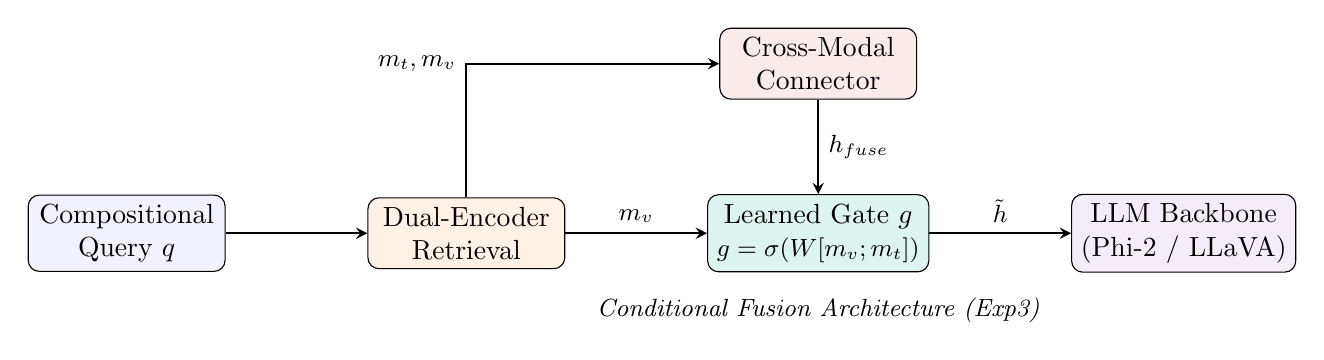
\begin{tikzpicture}[
      box/.style={draw, rounded corners, minimum width=2.5cm, minimum height=0.8cm, align=center},
      arr/.style={->, >=stealth, thick},
      node distance=1.2cm and 1.8cm
  ]
  \node[box, fill=blue!5] (query) {Compositional\\Query $q$};
  \node[box, right=of query, fill=orange!10] (retrieval) {Dual-Encoder\\Retrieval};
  \node[box, right=of retrieval, fill=memteal!15] (gate) {Learned Gate $g$\\ \small $g = \sigma(W[m_v; m_t])$};
  \node[box, above=of gate, fill=memred!10] (connector) {Cross-Modal\\Connector};
  \node[box, right=of gate, fill=mempurple!10] (llm) {LLM Backbone\\(Phi-2 / LLaVA)};

  \draw[arr] (query) -- (retrieval);
  \draw[arr] (retrieval) -- node[above, font=\small] {$m_v$} (gate);
  \draw[arr] (retrieval) |- node[left, font=\small] {$m_t, m_v$} (connector);
  \draw[arr] (connector) -- node[right, font=\small] {$h_{fuse}$} (gate);
  \draw[arr] (gate) -- node[above, font=\small] {$\tilde{h}$} (llm);

  \node[below=0.2cm of gate, font=\small\itshape] {Conditional Fusion Architecture (Exp3)};
  \end{tikzpicture}
  \caption{\textbf{Architecture overview for the Gated Connector (Exp3).} Instead of naive weighted sums, a learned gating layer dynamically decides whether to bypass the cross-modal connector based on the agreement between $m_v$ and $m_t$. This is strictly superior to unconditional baseline fusion.}
  \label{fig:architecture}
\end{figure}

\paragraph{Exp1: Adaptive Modality Gating (AMG).}
\textbf{Hypothesis:} Rule-based heuristics can dynamically lower the fusion weight when modalities conflict. We compute agreement $a = \cos(f_v(m_v), f_t(m_t))$. If $a < 0.6$, we reduce the fusion weight $\alpha$ from 0.9 to 0.5.

\paragraph{Exp2: Soft Top-$k$ Retrieval (STK).}
\textbf{Hypothesis:} Hard max-pooling amplifies near-miss boundaries. We replace top-1 selection with softmax-weighted interpolation over the top-$k$ neighbours (temperature $\tau=0.1$).

\paragraph{Exp3: Gated Connector (GC).}
\textbf{Hypothesis:} The connector must learn when \textbf{not} to fuse. We train a binary gate $g$ via a single linear layer over the concatenated memories:
\begin{equation}
  h_\text{out} = g \cdot \text{Connector}(m_v, m_t) + (1-g) \cdot m_v
\end{equation}
If $g=0$, textual memory is completely bypassed. The gate learns from task performance rather than heuristics.

\paragraph{Exp4: Confidence-Based Deferral (CBD).}
\textbf{Hypothesis:} In severe conflicts, deferring to human reviewers is safer. If the top-token generation probability $p < \tau_c$, the sample is flagged rather than answered.


%%%%%%%%%%%%%%%%%%%%%%%%%%%%%%%%%%%%%%%%%%%%%%%%%%%%%%%%%%%%

\newpage
% NeurIPS 2026 — Evaluation & Datasets Track Checklist
\section*{NeurIPS Paper Checklist}

\begin{enumerate}

\item {\bf Claims}
\item[] Question: Do the main claims made in the abstract and introduction accurately reflect the paper's contributions and scope?
\item[] Answer: \answerYes{}
\item[] Justification: The abstract and introduction state four contributions — Adversarial-2k dataset, failure taxonomy, evaluation protocol, and diagnostic analysis — all of which are described and evidenced in the paper body.
\item[] Guidelines: N/A

\item {\bf Limitations}
\item[] Question: Does the paper discuss the limitations of the work performed by the authors?
\item[] Answer: \answerYes{}
\item[] Justification: Section~\ref{sec:data_analysis} (Bias and Robustness) discusses dataset construction bias. Appendix notes on annotation guidelines discuss potential annotation artefacts.
\item[] Guidelines: N/A

\item {\bf Theory Assumptions and Proofs}
\item[] Question: For each theoretical result, does the paper provide the full set of assumptions and a complete proof?
\item[] Answer: \answerNA{}
\item[] Justification: This is a dataset paper. No new theoretical results are presented.
\item[] Guidelines: N/A

\item {\bf Experimental Result Reproducibility}
\item[] Question: Does the paper fully disclose all the information needed to reproduce the main experimental results of the paper to the extent that it affects the main claims and/or conclusions of the paper?
\item[] Answer: \answerYes{}
\item[] Justification: Section~\ref{sec:setup} fully describes model checkpoints, hyperparameters, and evaluation protocol. The dataset and code are released publicly.
\item[] Guidelines: N/A

\item {\bf Open access to data and code}
\item[] Question: Does the paper provide open access to the data and code, with sufficient instructions to faithfully reproduce the main experimental results, as described in supplemental material?
\item[] Answer: \answerYes{}
\item[] Justification: The dataset is available at \url{https://huggingface.co/datasets/MemEIC/CCKEB} under Apache 2.0. Code and evaluation scripts are released on GitHub.
\item[] Guidelines: N/A

\item {\bf Experimental Setting/Details}
\item[] Question: Does the paper specify all the training and test details (e.g. data splits, hyperparameters, how they were selected) necessary to understand the results?
\item[] Answer: \answerYes{}
\item[] Justification: Section~\ref{sec:setup} and Appendix~\ref{app:methods} provide full experimental details.
\item[] Guidelines: N/A

\item {\bf Experiment Statistical Significance}
\item[] Question: Does the paper report error bars suitably and correctly defined or other appropriate statistical significance measures for the experiments that support the main claims?
\item[] Answer: \answerYes{}
\item[] Justification: Section~\ref{sec:setup} states that all EA comparisons use paired bootstrap testing with 10{,}000 resamples.
\item[] Guidelines: N/A

\item {\bf Experiments Compute Resources}
\item[] Question: For each experiment, does the paper provide sufficient information on the computational resources (type of compute, computational time, memory requirements) for reproducing experiments?
\item[] Answer: \answerYes{}
\item[] Justification: Model sizes and GPU requirements are stated in Section~\ref{sec:setup}.
\item[] Guidelines: N/A

\item {\bf Code Of Ethics}
\item[] Question: Does the research conducted in the paper conform, in every respect, with the NeurIPS Code of Ethics?
\item[] Answer: \answerYes{}
\item[] Justification: All data sources are public-domain (Wikidata, COCO). No personal private data is used.
\item[] Guidelines: N/A

\item {\bf Broader Impacts}
\item[] Question: Does the paper discuss both potential positive societal impacts and negative societal impacts of the work performed?
\item[] Answer: \answerYes{}
\item[] Justification: The Conclusion discusses open challenges; dataset motivation discusses the societal need for reliable knowledge editing.
\item[] Guidelines: N/A

\item {\bf Safeguards}
\item[] Question: Does the paper describe safeguards that have been put in place for responsible release of data or models that have potential for misuse?
\item[] Answer: \answerYes{}
\item[] Justification: Adversarial filtering removes harmful content. Annotation quality control is described. No adversarial generation code is released in an exploitable form.
\item[] Guidelines: N/A

\item {\bf Licenses for existing assets}
\item[] Question: Are the creators or original owners of assets (e.g., code, data, models), used in the creation of your dataset/code/model, properly credited and are the license of the assets compatible with the license of your dataset?
\item[] Answer: \answerYes{}
\item[] Justification: COCO images are CC-BY; Wikidata is CC0; VLKEB-derived samples carry BSD-3 attribution. All are compatible with Apache 2.0.
\item[] Guidelines: N/A

\item {\bf New Assets}
\item[] Question: Are new assets introduced in the paper, e.g., code, dataset, models, documented and is the persistent URL provided?
\item[] Answer: \answerYes{}
\item[] Justification: Adversarial-2k is hosted on Hugging Face (\url{https://huggingface.co/datasets/MemEIC/CCKEB}). Code is on GitHub.
\item[] Guidelines: N/A

\item {\bf Crowdsourcing and Human Subjects}
\item[] Question: For crowdsourcing experiments and research with human subjects, does the paper include the information required under the respective Institutional Review Board (IRB)?
\item[] Answer: \answerNA{}
\item[] Justification: Annotation was conducted by expert in-house annotators, not via a crowdsourcing platform.
\item[] Guidelines: N/A

\item {\bf Informed Consent}
\item[] Question: Did the authors collect data from human subjects?
\item[] Answer: \answerNA{}
\item[] Justification: All data is derived from public-domain sources (COCO, Wikidata). No data was collected from human subjects.
\item[] Guidelines: N/A

\end{enumerate}


\bibliographystyle{unsrt}
\bibliography{refs}

\end{document}
